\documentclass[12pt]{article}
\usepackage[utf8]{inputenc}
\usepackage[left=1.5in, right=1in, top=1in, bottom=1in, includefoot, headheight=13.6pt]{geometry}
\usepackage[sorting=none]{biblatex}
\usepackage{graphicx}
\usepackage{amsmath}
\usepackage[center]{caption}
\usepackage{adjustbox}
\newtheorem{theorem}{Theorem}
\addbibresource{bib.bib}
\graphicspath{ {./figures/} }

\title{Network Complexity}
\author{Yipei Zhao}
\date{\today}

\begin{document}
\begin{titlepage}
    \begin{center}
        \vspace*{1cm}
            
        \Huge
        \textbf{Network Complexity}
            
        \vspace{0.5cm}
        \LARGE
        Thesis Subtitle
            
        \vspace{1.5cm}
            
        \textbf{Yipei Zhao}
            
        \vfill
            
        A dissertation presented for the degree of\\
        Master of Science
            
        \vspace{0.8cm}
            
        
\includegraphics[width=0.4\textwidth]{university.png}
            
        \Large
        MSc Data Analytics\\
        Aston University\\
        United Kingdom\\
        05 September 2021
            
    \end{center}
\end{titlepage}
\tableofcontents
\pagebreak
\section{Introduction}
In my literature review, several complexity measures were introduced, includes the theory and the difference between them. 
\subsection{Random graphs}
We have many real networks in the actual world, but defining or observing all of them is not feasible. For simulations and comparisons, network scientists introduced the idea of random networks. They are also known as Erdos-Renyi network in honour of two mathematicians: Paul Erdos and Alfred Renyi. They have important contributions to understand the properties of a random network\cite{barabási2016network}.\\
\noindent
There are two definitions of a random network:
\begin{itemize}
    \item $G(n,p)$ network. A network with $n$ nodes will be initialised, there will be at most $(n)(n-1)/2$ edges. Each edge will be instantiated with probability $p$. This approach brings a randomness property to the graph; number of edges $m$. A $G(n,p)$ graph returns a fixed $n$ but a different $m$ everytime. The expectation of $m$ is equal to $p(n)(n-1)/2$.
    \item $G(n,m)$ or $G(n,L)$ network. A graph with $n$ nodes will be initialised, $m/L$ edges will be connected from a random node to another random node. Due to the non-randomness of $G(n,m)$ networks, they are used to simulate the behaviour of a random network in this thesis. There will be also refered to random network/random graph in this report unless specified otherwise.
\end{itemize}

\noindent
In the literature review, we introduced the idea of clustering coefficient and average distance. For a random graph, the clustering coefficient and average distance can be calculated using formulas.\cite{barabási2016network} The average clustering coefficient of a random graph is $p$, or $2m/((n)(n-1))$(number of instantiated links divided by total number of possible links). Clustering coefficient is used to illustrate the ratio between connected links and possible links between a node's neighbours. If there are $k$ neighbours of a node, there can be at most $k(k-1)/2$ between the neighbours. In these $k(k-1)/2$ links, only $p$ of them will be instantiated. Thus, the ratio of connected links and possible links becomes $\frac{pk(k-1)/2}{k(k-1)/2}=p$. Additionally, average distance of a random graph $L_r \approx \frac{ln(n)}{ln\bar{(k)}}\approx \frac{ln(n)}{ln(2m/n)}$. To be noticed, both parameters are expectation/approximated, they won't be exact for a random graph.

\subsection{Rewiring}
\label{rewiring}
Except random graphs, network scientists desire alternative way to simulate real and random networks, which allows them to further study the nature and properties of networks. Network scientists would use a technique called rewiring to change the properties and parameters of a network, and monitor the change of parameters respect to the rate of rewiring.\cite{network_rewiring} In this report, we are going to introduce two simple rewiring technique:single link rewiring and pairwise rewiring.\\
\begin{itemize}
    \item Starting with an edge $(u,v)$; with starting node $u$ and ending node $v$. Single link rewiring will look for a node $w$ that hasn't yet been connected to node $u$. Once $w$ is found, edge $(u,v)$ will be removed and a new link $(u,w)$ will be added to the network. 
    \item Starting with two edge $(u,v)$ and $(x,y)$. Pairwise rewiring will remove both edges, and two new edges will be added in: $(u,y)$ and $(x,v)$.
\end{itemize}
\noindent
Single link rewiring tends to give higher randomness to the network, and pairwise rewiring preserves the degree distribution. Rewiring usually requires a parameter $p$, which is the probability of rewiring for each edge. If $p=1$, using single link rewiring will cause the network to become a random network. However, since pairwise rewiring preserves the degree detribution, $p=1$ will not cause the network to become completely random.

\subsection{Small-world}
\label{small_world}
About 50 years ago, a famous study was carried out by Standley Milgram\cite{milgram1967small} in the interest of this question: how many intermediates are needed to pass a message between two irrelevant or distnaced person? This is known as the small-world problem. As counterintuitive as it may seem, the medium number of intermediates needed is only 5(an average of 6). This is not a fair and undoubtable experiment and it is almost impossible to determine the actual number of intermediates needed in mordern world. Nevertheless, this number would be smaller than most peoples' expectation. Mathematically, the small world problem is the study of graphs with small path length. Previously, we introduced the formula to calculate the average distance $L_r$ of a random graph. Thus, if a graph has $L/L_r <1$, this graph has less average distance than random graphs. If the ratio $L/L_r$ is relatively small, we can classify it as a small-world network.\\
\noindent
A small-world network can be generated by a Watts-Strogatz(WS) model\cite{wsmodel} or a Newman-Watts(NW) model(a variant of the WS model)\cite{nwmodel}. Both models require three parameters: number of nodes $n$, number of connected closest neighbours $k$ and rewiring probability $p$. The key of both model is rewiring(single link rewiring). The graph starts with $n$ nodes, each node is connected to $k$($k-1$ if $k$ is odd) nearest neighbours; $nk/2$ edges will be created. For each edge $(u,v)$, there is a probaiblity $p$ the a new edge $(u,w)$ is created(maintains the starting node but connects to another random node). While rewiring, the WS model removes the edge $(u,v)$, thus, the number of edges stays the same. However, the NW model maintains the edge $(u,v)$, causing the expectation of number of edges after rewiring to be $nk/2+pnk/2$. Rewiring will add short path to the networks, and cause the average distance to be exceptionally smaller. Suggested by Barabasi\cite{barabási2016network}, to obtain both high clustering and low average distance, $p$ should be between 0.001 and 0.1.\\

\begin{figure}[ht]
    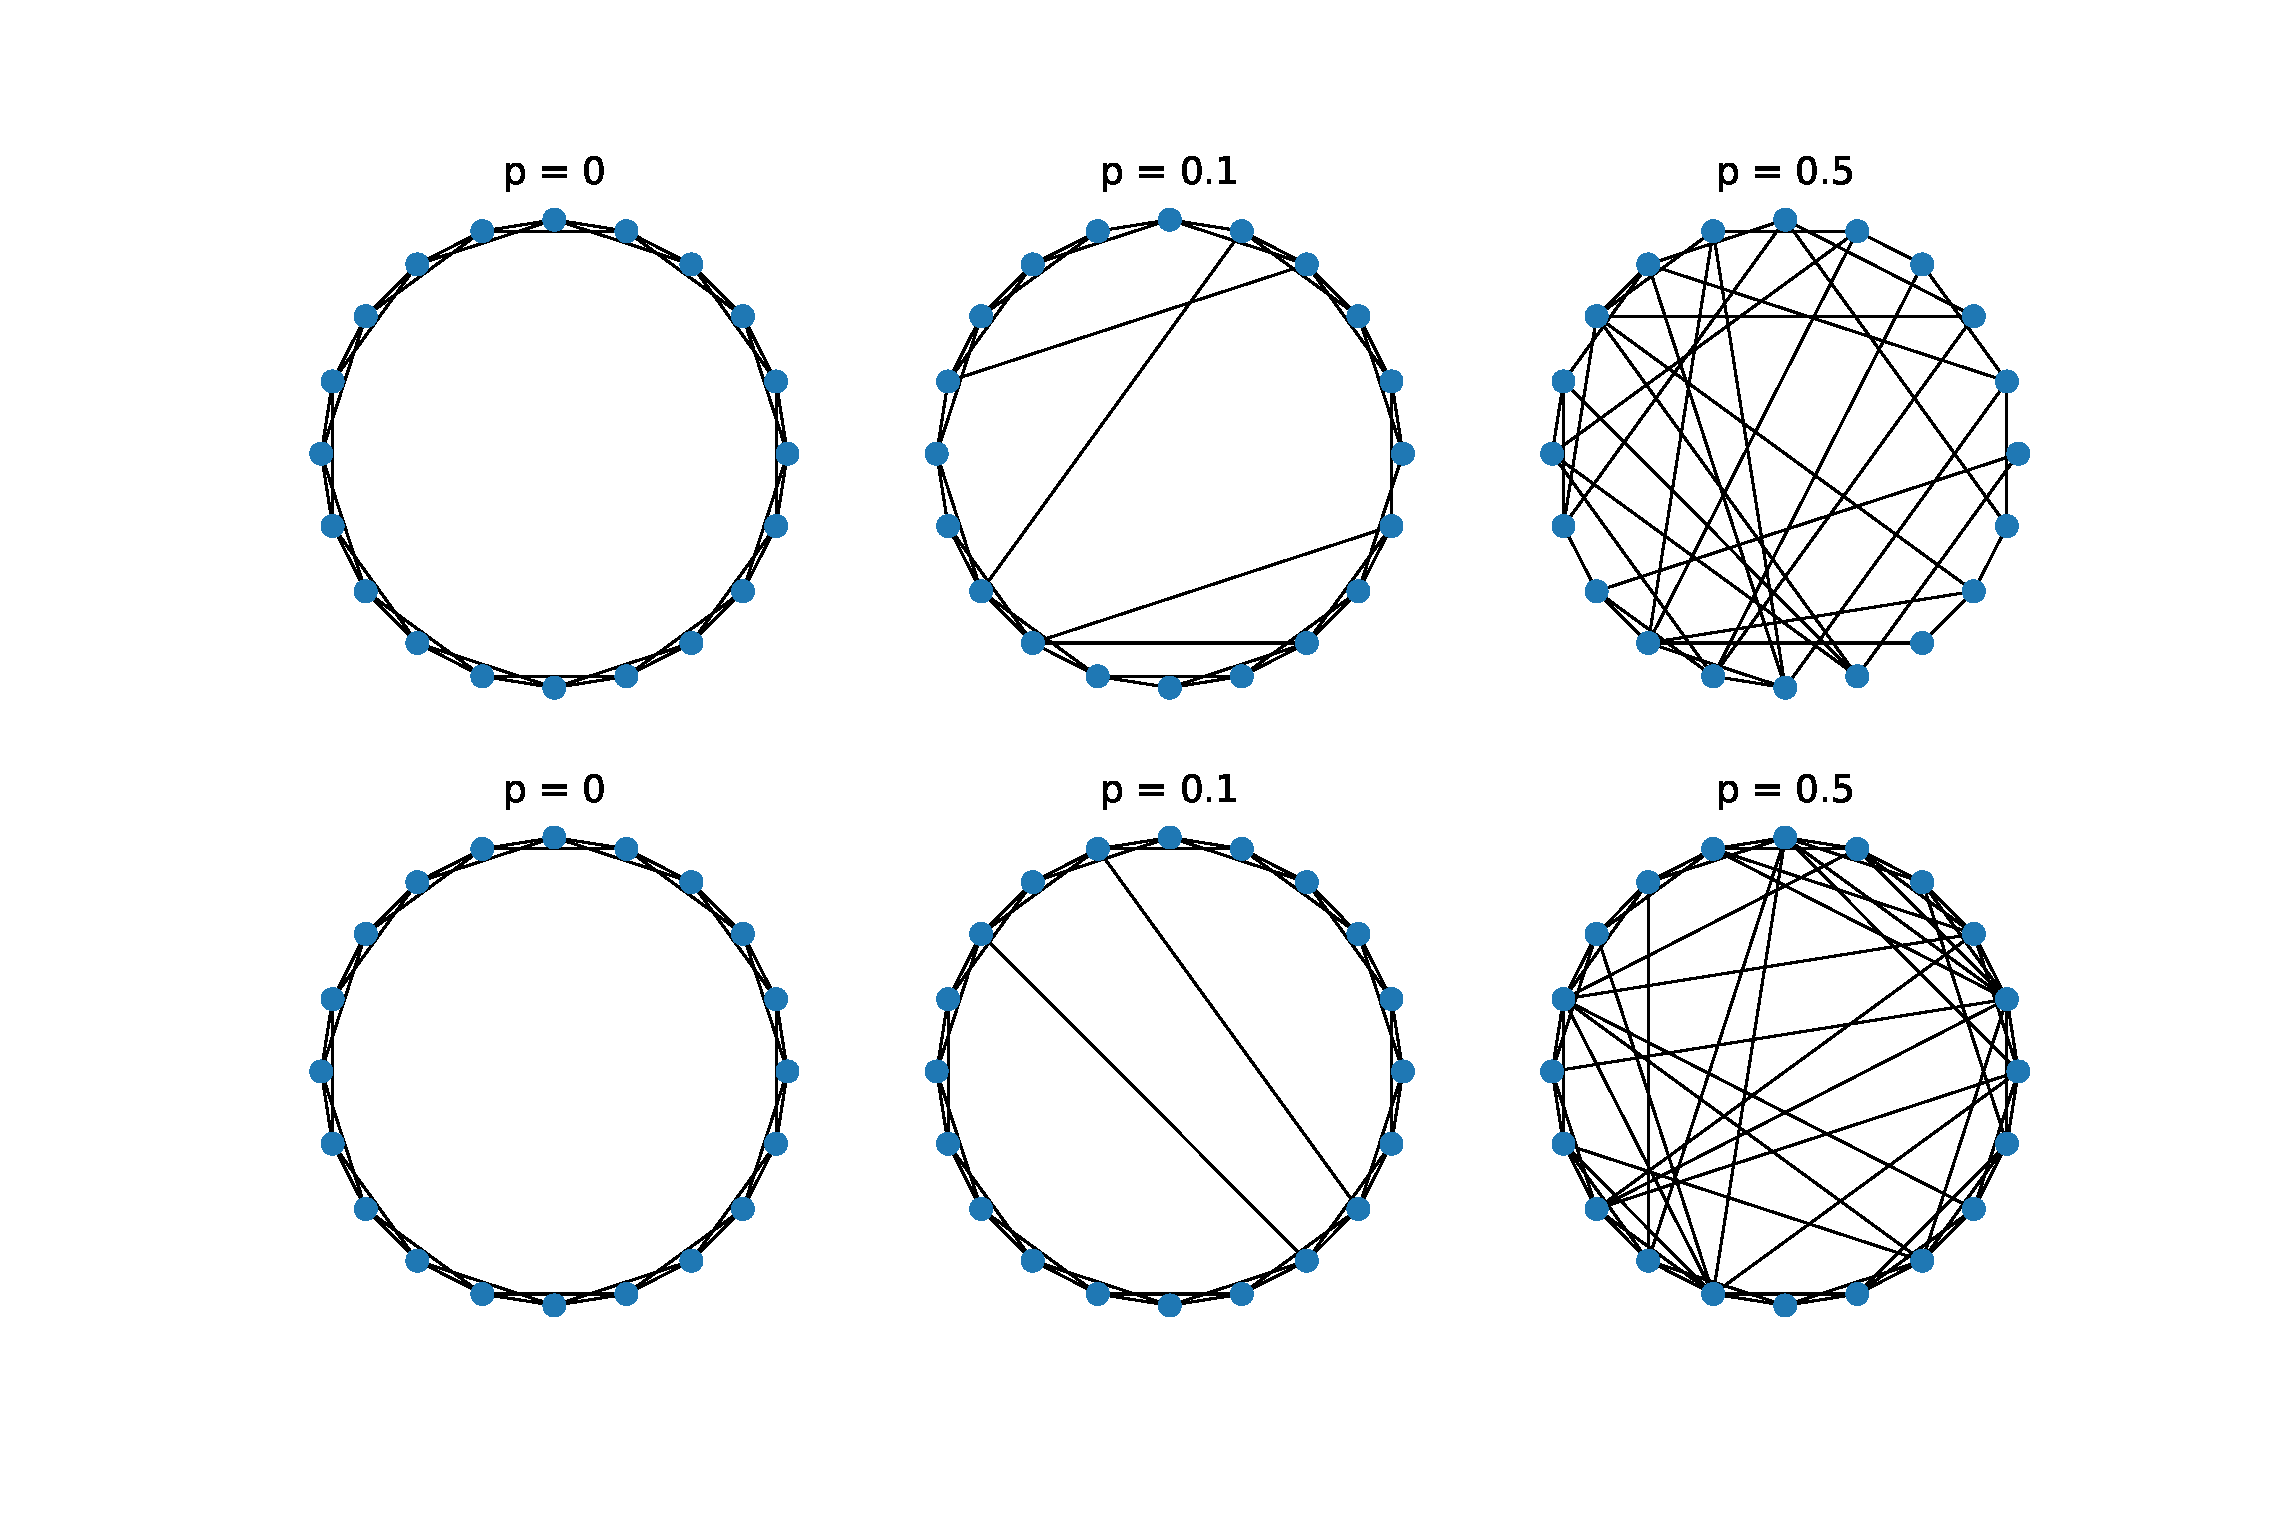
\includegraphics[width = \textwidth]{small_world_network_model.eps}
    \centering
    \caption{A demonstration of WS model and NW model. The paramters are: $n=20$, $k=4$, $p=0,0.1,0.5$.}
    \label{fig:small_world_models}
\end{figure}

\subsection{Scale-free network}
A controversial topic of network science is wether real networks are usually scale-free. To state the definition of scale-free, we need to scope into the degree distribution of graphs.\\

\begin{figure}[ht]
    \centering
    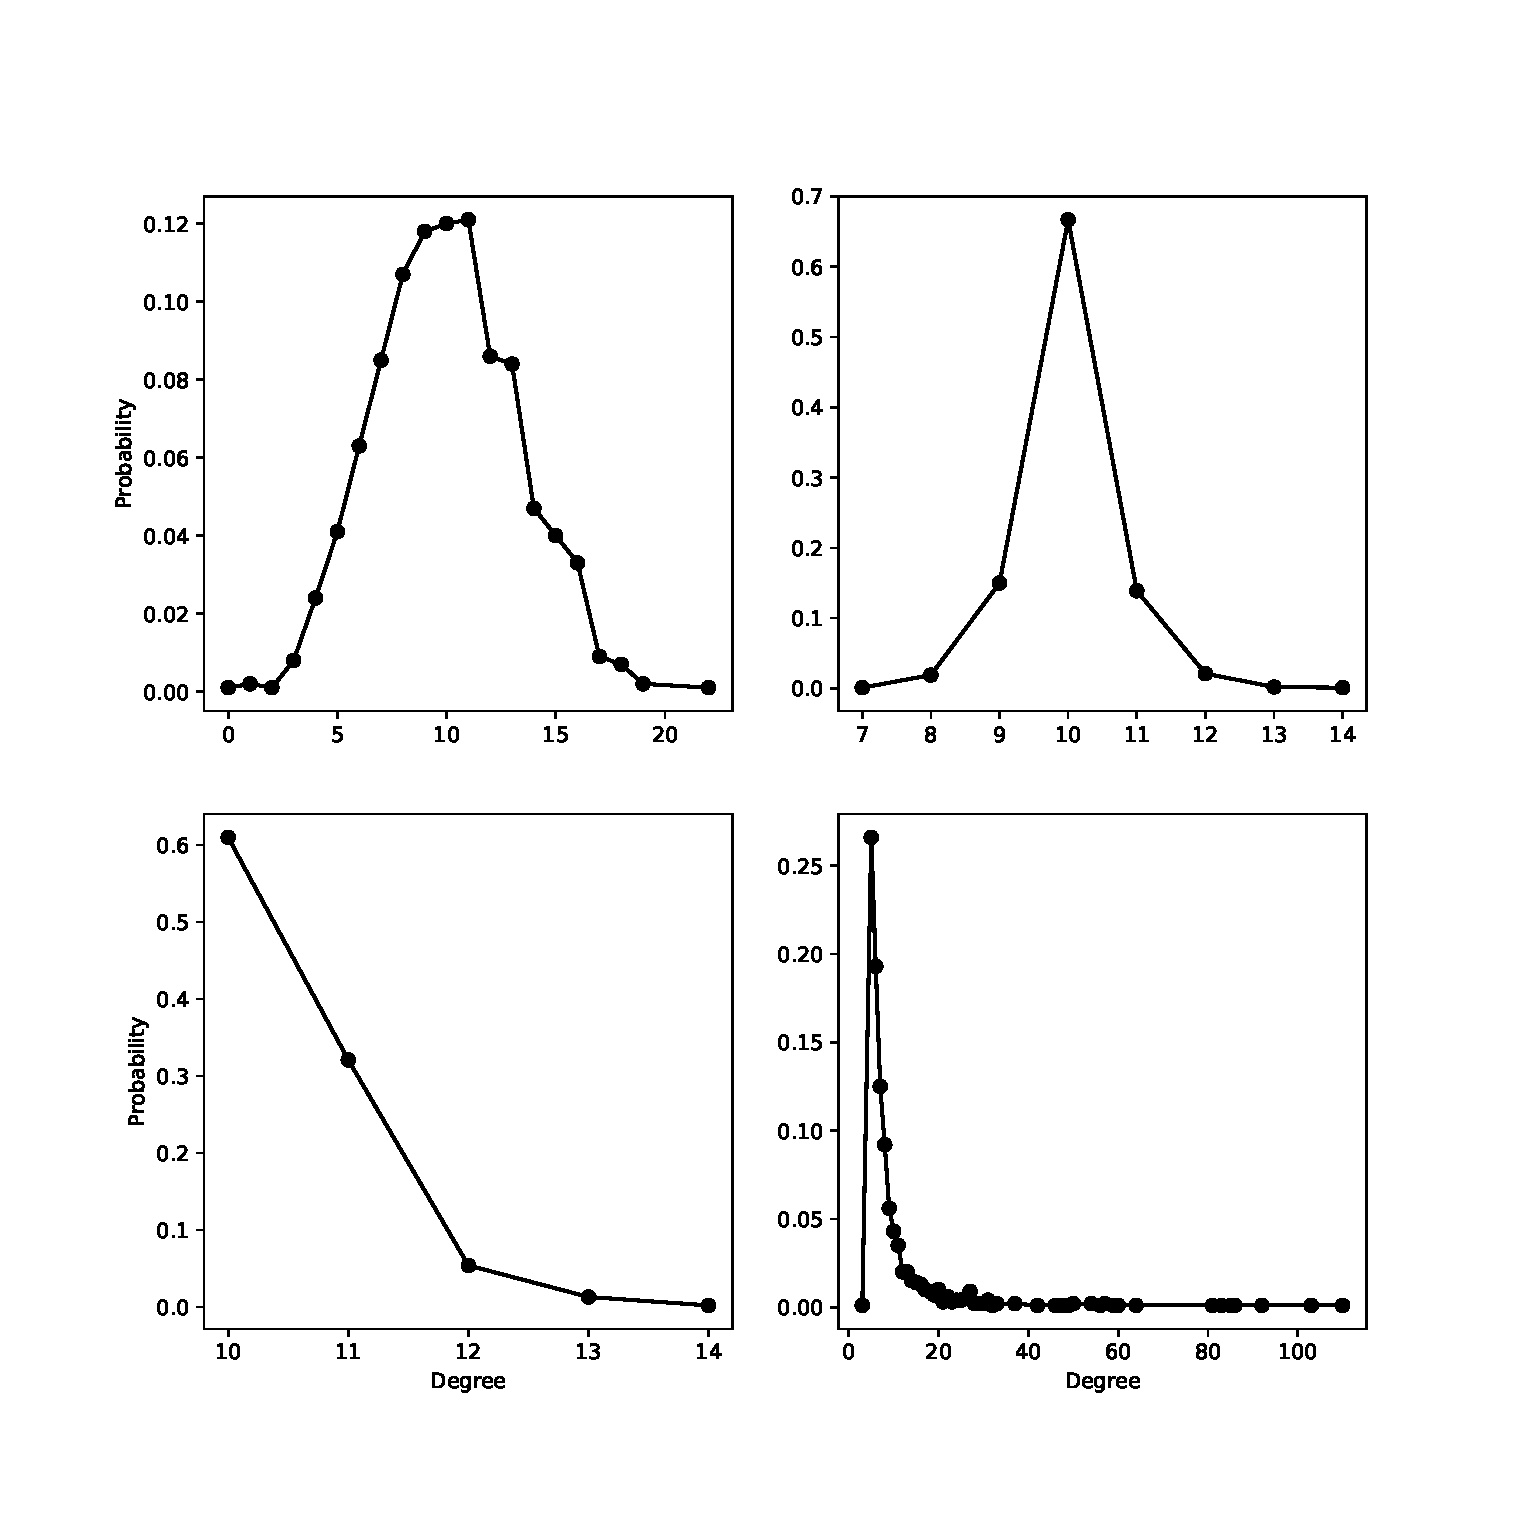
\includegraphics[width=\textwidth]{degree_distribution.eps}
    \centering
    \caption{Degree distribution of a $G(n,m)$ graph with $n=1000,m=5000$ and a graph generated by Barabasi-Albert model with $n=1000,m=5$.}
    \label{fig:degree_dist}
\end{figure}
\noindent
Suggested by Barabasi\cite{barabási2016network}, the degree distribution of a random graph is expected to follow a Poisson distribution. However, Poisson distribution is not the ideal distribution of a real network. A controversial idea that hasn't yet been proven in network science community is: are real networks' degree distribution follows a power-law distribution?\cite{broido_clauset_2019} A power-law distribution follows: $P(k) \sim k^{-\gamma }$, the parameter $\gamma$ is typically in the range $2<\gamma<3$. If the degree distrution of a graph follows power-law distribution, the graph is said to be a scale-free network. Even though there are counter-examples, many network scientists still believe that real networks are scale-free. In order to further simulate the behaviour of real networks, Barabasi introduced the Barabasi-Albert(BA) model to create scale-free networks.\cite{barabási2016network}.\\
The BA model requires two parameters: $n$ and $m$. Initally, only one node is created. Whenever a node is added into the network, it will connect to $m$ nodes. The logic of connection is the key of this model. Nodes are more likely to connect to nodes with more links than nodes with less links. For instance, a node has been added to the network, it is more likely to connect to a node with 7 links than a node with 3 links. This logic of connection is called preferential attachment. Essentially, like in real world, nodes are more likely to connect to another node that has more impact on the network. The BA model ensures most of the nodes have low degree, whereas only a few nodes have exceptionally high degree, as shown in figure \ref{fig:degree_dist}. An ideal way to fit the power-law distribution is using a linear regression to fit the data in log-log scale.

\subsection{Generated graphs}
\label{generate_graphs}
All graph generators are utilized as below(unless specified):
\begin{itemize}
    \item $G(n,m)$ random graphs/networks or random graphs/networks. With given $n$, $m$ will be randomly selected between $n-1$ to $n(n-1)/2$.
    \item For WS and NW graphs, three parameters are required. Given parameter $n$, $k$ will be randomly selected between 1 and $(n-1)$. $p$ is also randomize, within the range 0.01 and 0.1 to simulate small-world network as mentioned in section \ref{small_world}.
    \item Two parameters are needed for BA graphs, given $n$, $m$ will be randomize between 1 and $(n-1)$.
\end{itemize}

\section{Methods}
\subsection{Implemeted methods}
In the literature review, 9 methods were introduced, 7 methods were succesfully implemented and tested with a new method $MAri$ based on the idea of $MAg$. The implemented methods are:
\begin{itemize}
    \item Subgraph measures:
    \begin{itemize}
        \item $C_{1e,st}$
        \item $C_{1e,spec}$
        \item $C_{2e,spec}$
    \end{itemize}
    \item Product measures:
    \begin{itemize}
        \item $MAg$
        \item $MAri$
        \item $Cr$
        \item $Ce$
    \end{itemize}
    \item $OdC$ (Entropy measure)
\end{itemize}

\subsection{$MA_{RI}$}
The $MAg$ measure is a product measure, which distributes higher complexity to graphs with medium number of edges and lower complexity at both tails. Using the product of redundancy $R$ and mutual information $I$, with normalisation, $MAg$ is defined as\cite{KIM20082637}:
\begin{equation}
    \label{eq:RandI}
    \begin{gathered}
        R = \frac{1}{m}\sum_{i,j>i}ln(d_id_j)\\
        I = \frac{1}{m}\sum_{i,j>i}ln(\frac{2m}{d_id_j})\\
    \end{gathered}
\end{equation}
\begin{equation}
    \label{eq:mag}
    \begin{gathered}
        MA_R = 4(\frac{R-R_{path}}{R_{clique}-R_{path}})(1-\frac{R-R_{path}}{R_{clique}-R_{path}})\\
        MA_I = 4(\frac{I-I_{clique}}{I_{path}-I_{clique}})(1-\frac{I-I_{clique}}{I_{path}-I_{clique}})\\
        MA_g = MA_R * MA_I
    \end{gathered}
\end{equation}
$I$ can be written as:
\begin{equation}
    \label{eq:mutual_info}
    \begin{gathered}
        I = \frac{1}{m}\sum_{i,j>i}ln(\frac{2m}{d_id_j})\\
        I = \frac{1}{m}(\sum_{i,j>i}ln(2m)-\sum_{i,j>i}ln(d_id_j))\\
        I = \frac{1}{m}\sum_{i,j>i}ln(2m)-\frac{1}{m}\sum_{i,j>i}ln(d_id_j)\\
        I = ln(2m)-R
    \end{gathered}
\end{equation}
\noindent
$R_{path},R_{clique},I_{path}$ and $I_{clique}$ represent the lowest redundacy, highest redundancy, highest mutual information and lowest mutual information of graphs with fixed $m$ and $n$ respectively. The equations can be found in the literature review. Kim and Wilhelm suggested that network scientists may use $C=(R-R_{path})(I-I_{clique})$ as a complexity meassure, however, the upperbound cannot be found to normliase the complexity. From our study, an upper-bound of $C$ can be calculated analytically.\\
Assuming the upper-bound $C_{max}$ can be found, $0<C/C_{max}<1$. As suggested in equation set \ref{eq:mutual_info}, $I = ln(2m)-R$, we can rewrite the complexity equation:\\
\begin{equation}
    \label{eq:rewrite_complexity}
     C = (R-R_{path})(ln(2m)-R-I_{clique})\\
\end{equation}
\begin{equation}
    \label{eq:rewrite_complexity_1}
    C = -R^2+(ln(2m)-I_{clique}+R_{path})R+(-R_{path}ln(2m)+R_{path}I_{clique})
\end{equation}
By observing equation \ref{eq:rewrite_complexity_1}, we can conclude that the complexity function is a quadratic function, which means, there is one and only one extrema. Considering the nature of complexity measure, it's safe to assume that the extrema is a maxima. To find the extrema, we can differentiate the function respect to $R$ where the function's slope is 0:
\begin{equation}
    \label{eq:mari_diff}
        \frac{dC}{dR} = -2R_{max}+ln(2m)-I_{clique}+R_{path} = 0\\
\end{equation}
\begin{equation}
    \label{eq:rmax}
    R_{max} = \frac{ln(2m)-I_{clique}+R_{path}}{2}
\end{equation}
\noindent
We found $R_{max}$ where $C$ reaches its maxima. 
Substitutes equation \ref{eq:rmax} into equation \ref{eq:rewrite_complexity}:\\
\begin{equation}
    \begin{gathered}
        C_{max} =(R_{max}-R_{path})(ln(2m)-R_{max}-I_{clique})\\
        C_{max} = (\frac{ln(2m)-I_{clique}+R_{path}}{2}-R_{path})(ln(2m)-\frac{ln(2m)-I_{clique}+R_{path}}{2}-I_{clique})\\
        C_{max} = (\frac{ln(2m)-I_{clique}-R_{path}}{2})(\frac{ln(2m)-R_{path}-I_{clique}}{2})\\
    \end{gathered}
\end{equation}
\begin{equation}
    \label{c_max}
    C_{max} = \frac{(ln(2m)-I_{clique}-R_{path})^2}{4}
\end{equation}
\noindent
Thus, using equation \ref{c_max}, we can define a new measure $MA_{RI}$, which is defined by $C/C_{max}$:\\
\begin{equation}
    MA_{RI} = \frac{4(R-R_{path})(I-I_{clique})}{(ln(2m)-I_{clique}-R_{path})^2}
\end{equation}
\noindent
The complexity of $MA_{RI}$ is identical to $MA_g$, which can be calculated in $O(m)$ time.\\
As shown in figure \ref{fig:mariandmag}, $MA_{RI}$ gives higher coplexity to sparser graphs but less complexity when approaching to medium number of links. Additionally, it decreases almost linearly with $m$ once the peak is reached.
\clearpage
\begin{figure}[ht]
    \label{fig:mariandmag}
    \centering
    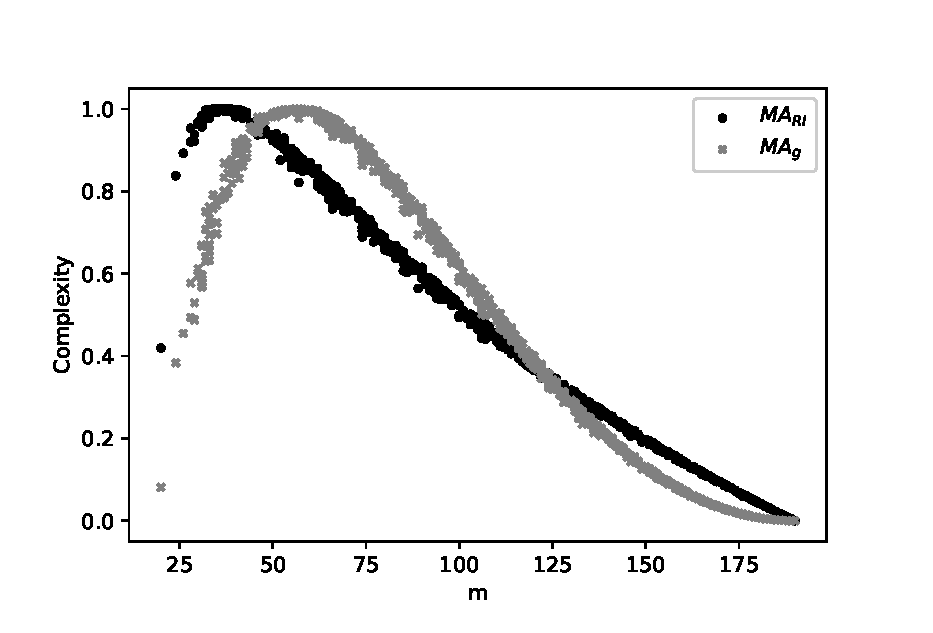
\includegraphics[width=\textwidth]{mariandmag.eps}
    \caption{$MA_g$ and $MA_{RI}$ complexity of $G(n,m)$ models, where $n=20$ and 1000 samples with random $m$ have been generated.}
\end{figure}

\subsection{Potential problems and solutions of different subgraph measures}
\label{problem}
During the implementation of measures, several problems were found, possible solutions are also given for future discussions.\\
Different subgraph measures are principally simple, but they are complex to compute, within at least $O(n^2)$ time\cite{KIM20082637}. This is not the only problem. An upper-bound of the complexity $m_{cu} = n^{1.68}-10$ was introduced by Kim and Wilhelm\cite{KIM20082637} to normalise the complexity. However, from the simulation, we found that this may not be the actual upper-bound of the different subgraph measures.

\begin{figure}[ht]
    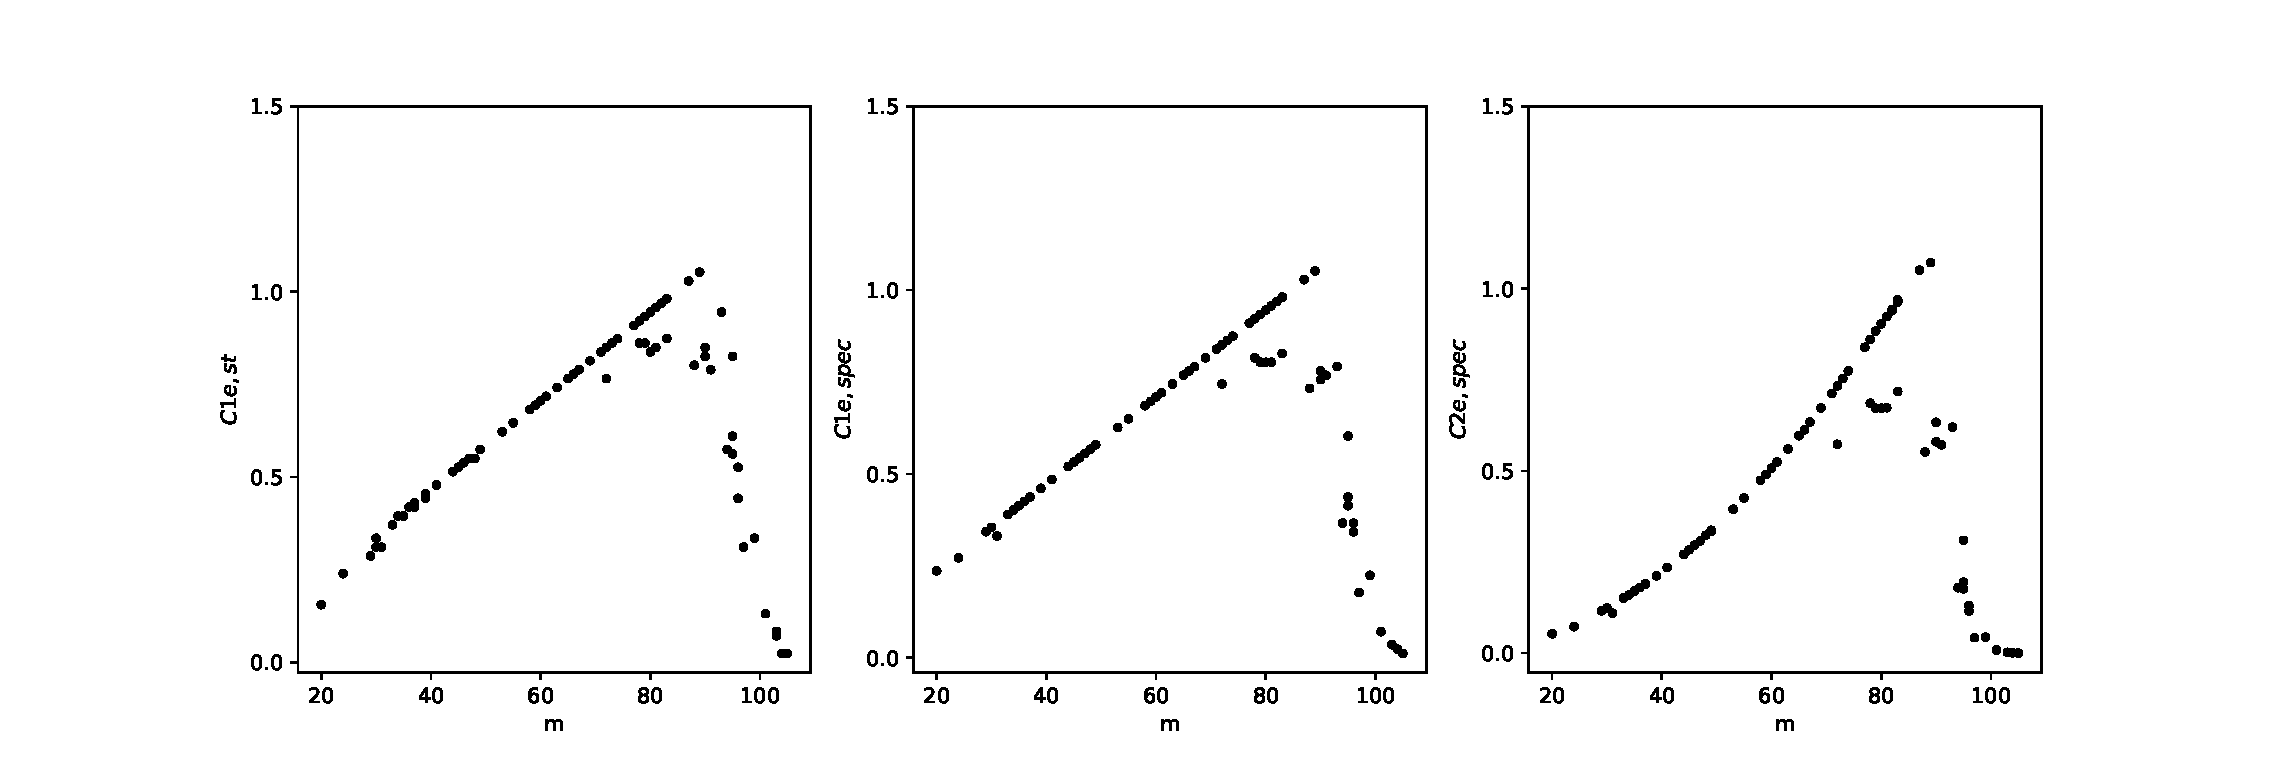
\includegraphics[width=\textwidth]{subgraph_measures.eps}
    \caption{Different subgraph measure of $G(n,m)$ random graphs, with $n$ = 15.}
    \label{fig:subgraph_measure}
\end{figure}
\noindent
The complexity is abnormal for graphs with around 90 edges and 15 nodes as shown in figure \ref{fig:subgraph_measure}. This could imply that the upper-bound assumption $m_{cu}$ is not correct, but there is another possible reason, which is the problem of floating point arithmetic.\\
On most machines today, numbers are represented in binary system\cite{floating_point}. For example, 0.2 is 0.00110011001100110011... in a binary system. This series is infinite, represented by $1*2^{-3}+1*2^{-4}+1*2^{-7}+1*2{-8}...$. For obvious reasons, computer scientists don't want to work with infinite series, therefore, the series is approximated. On a modern compueter, the series is usually approximated to 63 digits with 1 digit represents the sign of the number. After approximation, the error could cause the equal operation to fail in programming languages. A well known example is that for modern programming language or machine that operates this numbering system, 0.2+0.1 does not equal to 0.15+0.15. As a result, the comparison may cause more number of different subgraph than actual.\\
The core of different subgraph measure is to compare the cofactor($C_{1e,st}$)/spectrum($C_{1e,spec}$ and $C_{2e,spec}$) of a subgraph. Given the fact that the proabbility of a decimal number to appear in the sprectrums is high and the cofactor will also be very large for a large graph. The comparisons will be inaccurate. There are three possible solutions:
\begin{itemize}
    \item As suggested, errors will be made when approxiamted by the machine. An error threshold can be used when comparing spectrums and cofactors. For example, two numbers with relative error less than 1\% can also be considered as equal numbers. One disadvantage is the increase of complexity, taking more time and effort to compare the spectrums/number of spanning trees.
    \item Similarly, numbers can be rounded before comparison to avoid error. This is used in the implementation of different subgraph measures, all cofactors and spectrums are rounded to first 10 significant figures. This solution requires less computation time than first solution. The drawback is that similar graphs can be considered as isomorphic graphs, this also applies to the first provided solution, but with higher accuracy for large graphs. This may still gives complexities larger than 1, but it is the best solution considering the efforst spent.
    \item Instead of using $m_{cu}$ as a normalisation parameter, $m$ or $n(n-1)/2$ can be used for one-edge-deleted subgraph complexity and $\genfrac(){0pt}{2}{m}{2}$ for two-edges-deleted subgraph complexity. This gurantees the normalisation and avoid the mistake that caused by the first two solutions, but on the other hand, causing the complexity to be different.
\end{itemize}
A unique problem with $C_{2e,spec}$ is the value is not properly normalised for small graphs.

\begin{figure}[ht]
    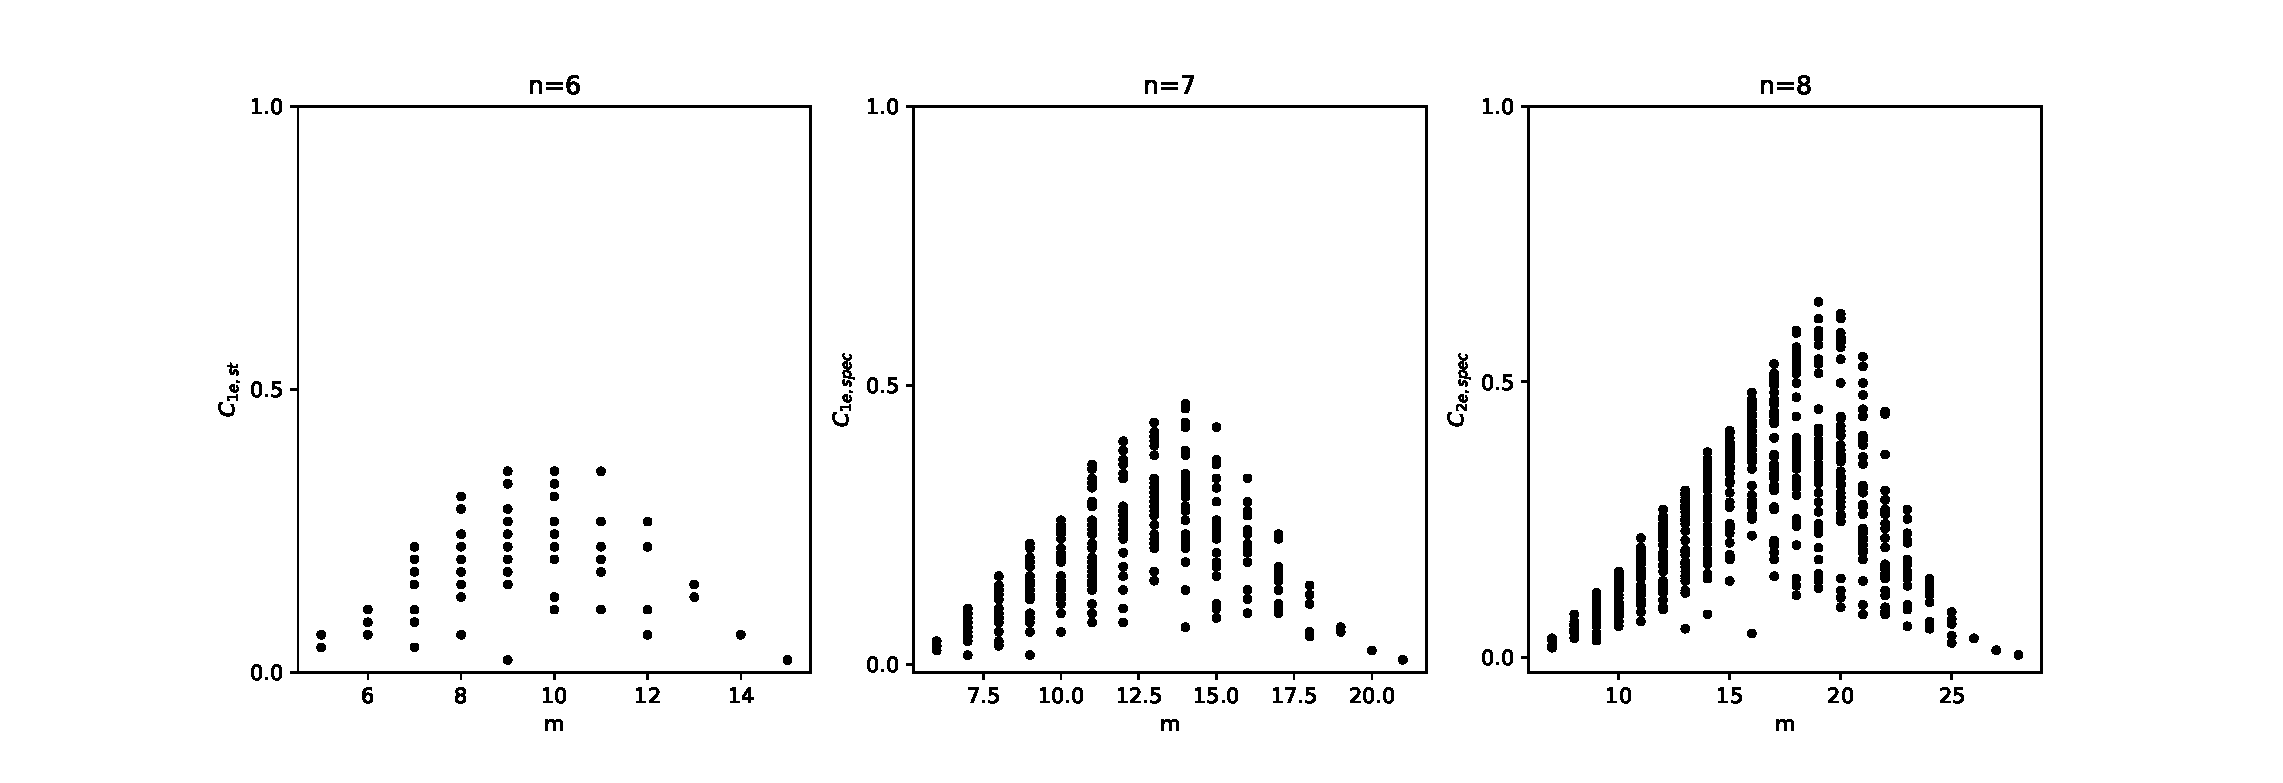
\includegraphics[width = \textwidth]{c2espec.eps}
    \caption{$C_{2e,spec}$ complexities for n = 6,7,8 respectively.}
    \centering
\end{figure}
\noindent
The upper-bound of $C_{2e,spec}$ is 0.5 while $ n\leq7 $. To have an upper-bound at 1, the complexity values have to be scaled by 2. However, scale by 2 will cause the complexity to exceed 1 for larger graphs. Thus, we sticked to the original normalisation and $C_{2e,spec}$ will have an upperbound at 0.5 for $n \leq 7$.

\section{Result}
\subsection{Complexity measures on small random graphs}
To test the performance of implemented measures, we tried all meausres on $G(n,m)$ random graphs with $n=7$ where 50 samples are generated for each $m$. As shown in figure \ref{fig:small_graphs}, we reproduced results as Kim and Wilhelm did in \cite{KIM20082637}. Except $C_{2e,spec}$, as mentioned in section \ref{problem}, there is a scaling problem. Most of the methods reaches its maximum with medium number of links. Low complexity are given to highly connected graphs and relatively sparse graphs.
\\
Different subgraph measures perform similarly, there is a big difference between the maximum and minimum with same $m$. Thus, it is very difficult to predict the complexity of a graph with given $m$ and $n$. The highest complexity is reached at $m=15$ for $C_{1e,st}$ and $C_{1e,spec}$ and $m=14$ for $C_{2e,spec}$. There is a miss in the plot: $C_{1e,spec}$ and $C_{2e,spec}$ plot does not contain a data point at (6,0). There is a very small proabbility for $G(n,m)$ model to generate a star graph(n-1 nodes are connected to 1 node, in total of n-1 edges), which will result in 0 complexity using $C_{1e,spec}$ and $C_{2e,spec}$ measure. We recommend to use different subgraph measure for small graphs as it is relatively independent of $m$, but not for large graphs due to its complexity.\\
$OdC$ is highly based on the degree distribution of a graph.\cite{odc} Thus, it spreads across the space and has little relationship with $m$. $OdC$ assigns a lot of graphs with 6 edges high complexity than desired. $OdC$ is "hierarchy sensitive", it may not create big difference between graphs when the graphs are small.\\
All 4 product measures are similar, gives higher complexity value at medium number of edges and less at both tails. There is a very small difference between graphs with same number of edges. $Ce$ and $Cr$ tends to give highest complexity to graphs with exactly $n(n-1)/4$ edges, and $MA_{RI}$ and $MA_{g}$ reach their maximum before medium number of edges as expected. Product measure are highly depending on $m$, one may guess the complexity of a graph solely based on $m$ and $n$. Network scientists may use machine learning techniques to approximate the complexity of a graph using $m$ and $n$, to calculate the complexity in an extremly small amount of time. On the other hand, product measure may not be optimal because a complexity measure should not solely based on $m$ and $n$, but the overall structure of a network.
\begin{figure}[ht]
    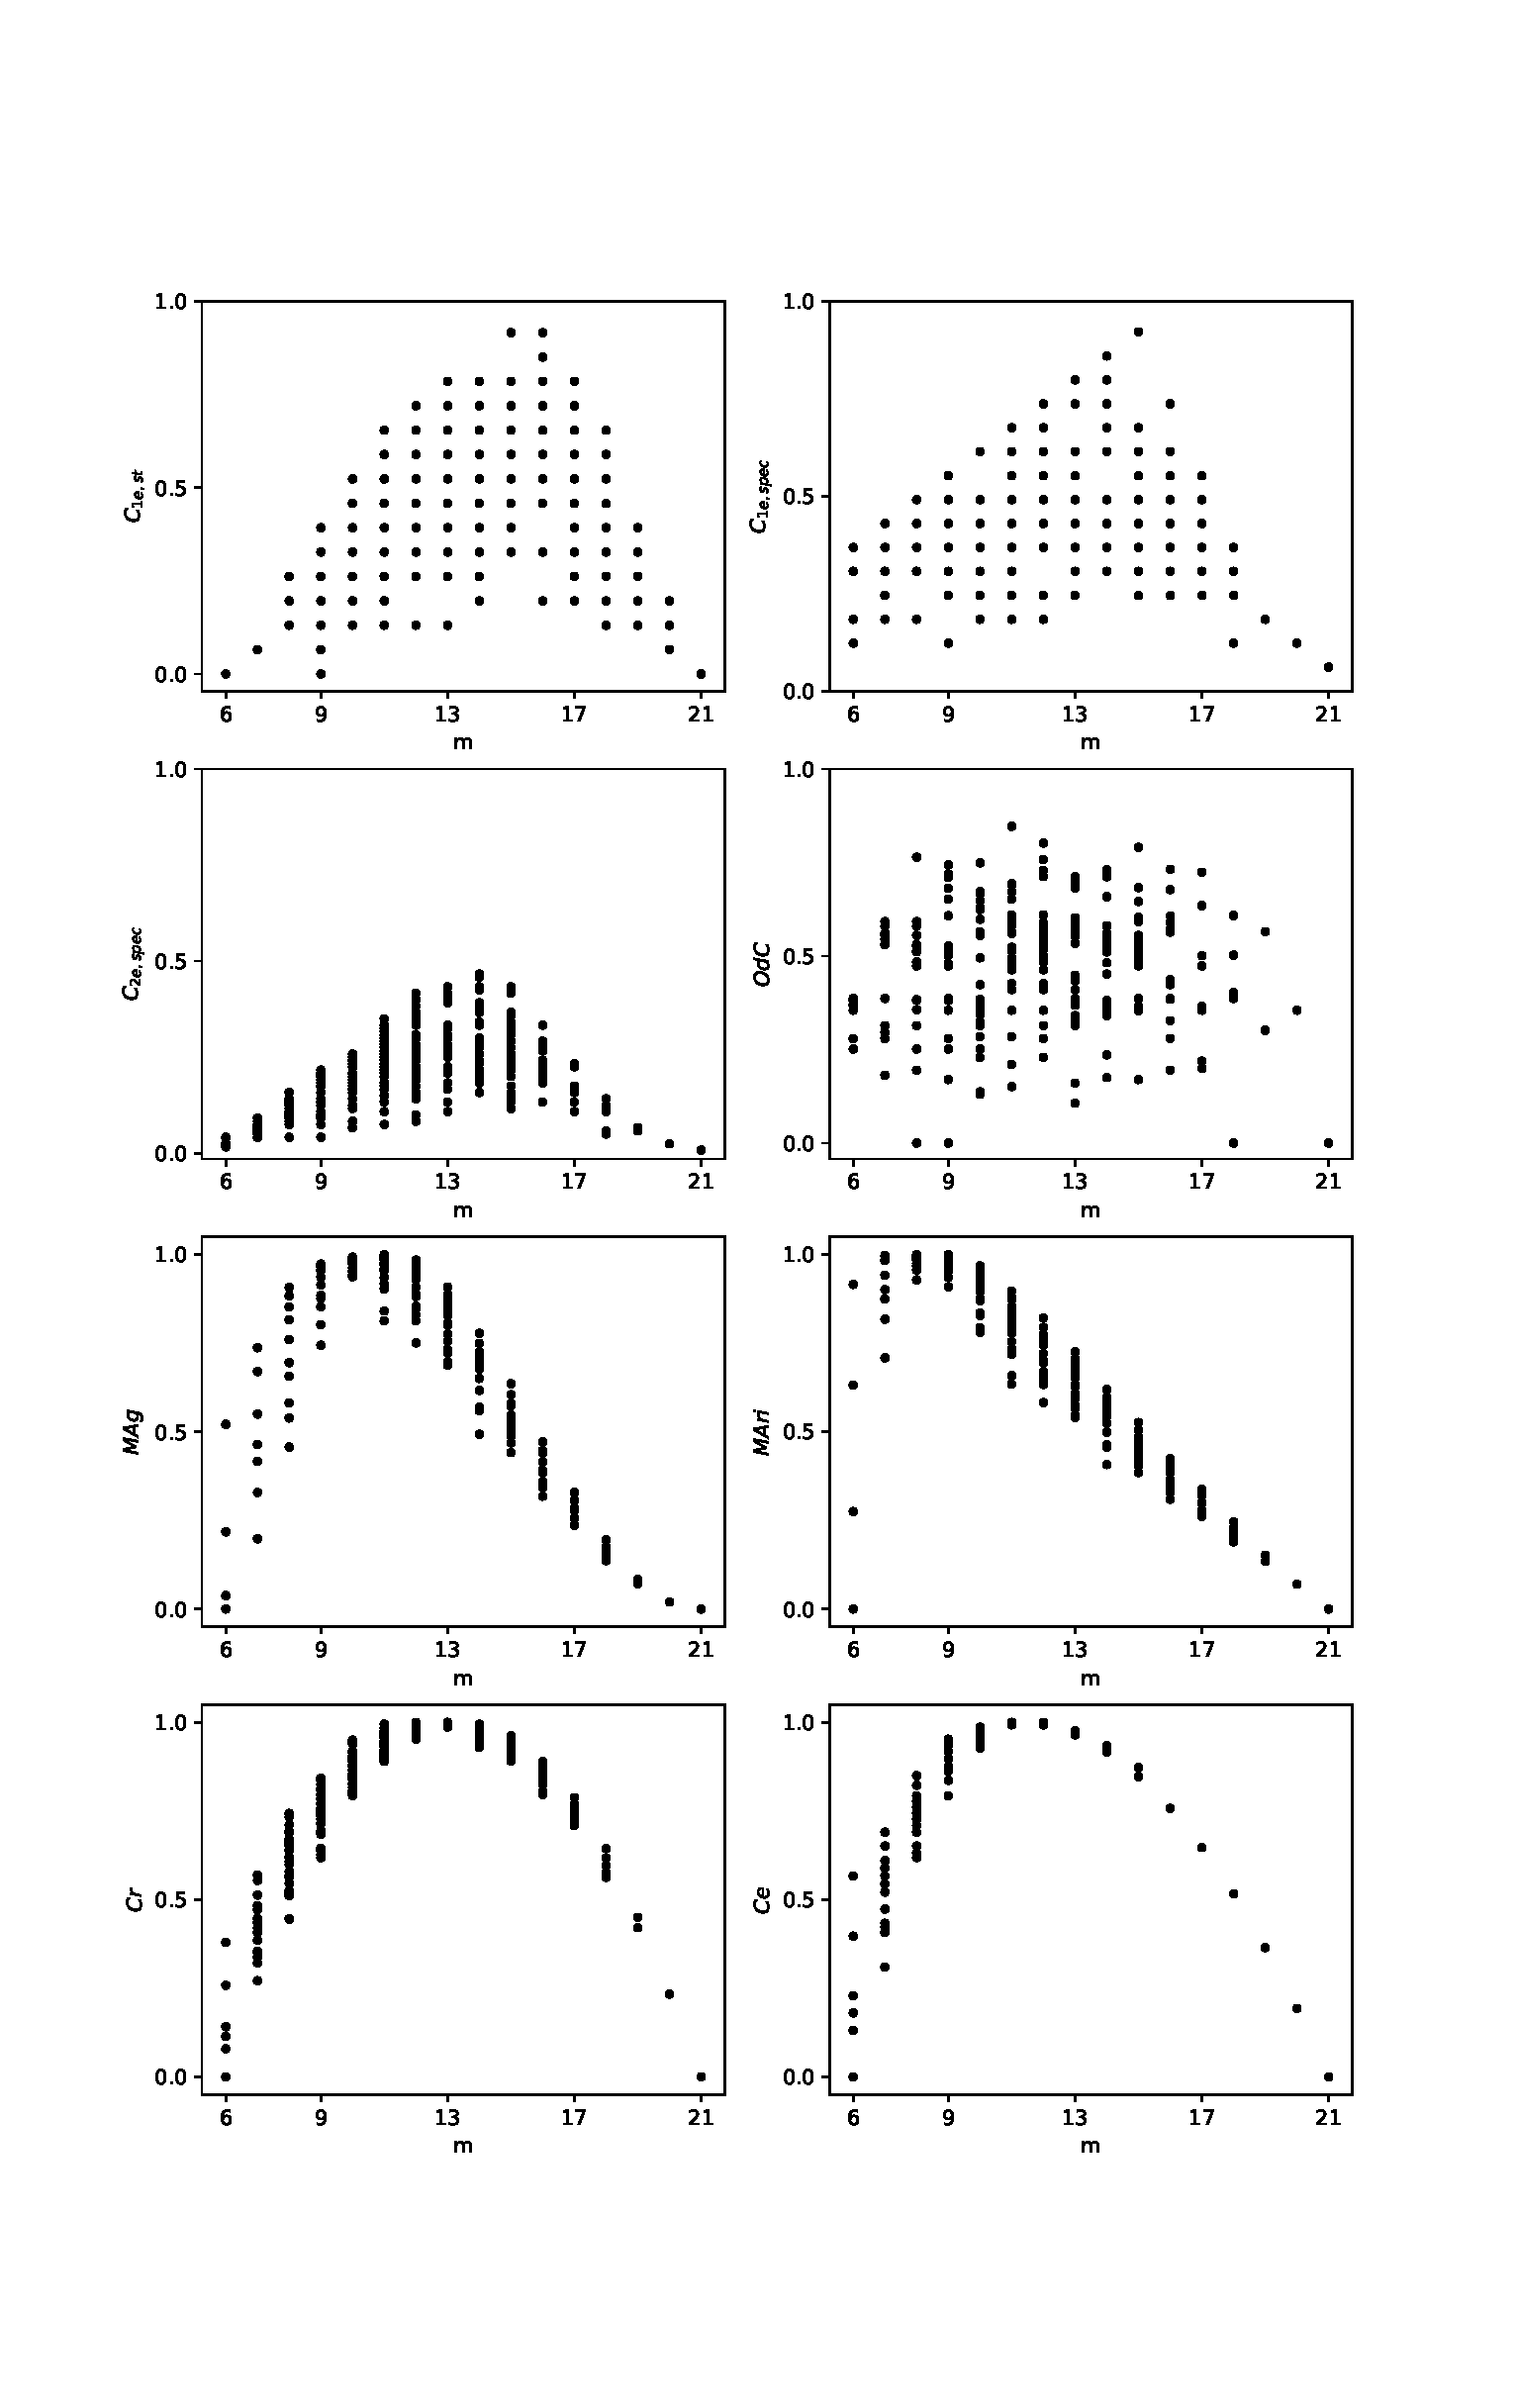
\includegraphics[width=0.7\textwidth]{complexities.eps}
    \centering
    \caption{Complexity of graphs generated using $G(7,m)$ model, 50 samples are generated for each $m$. Methods from top-left to bottom-right are: $C_{1e,st}$, $C_{1e,spec}$, $C_{2e,spec}$, $OdC$, $MAg$, $Cr$, $Cr$ and $MAri$.}
    \label{fig:small_graphs}
\end{figure}

\subsection{BA,WS and NW model}
\label{complexity_sp}
\begin{figure}[ht]
    \centering
    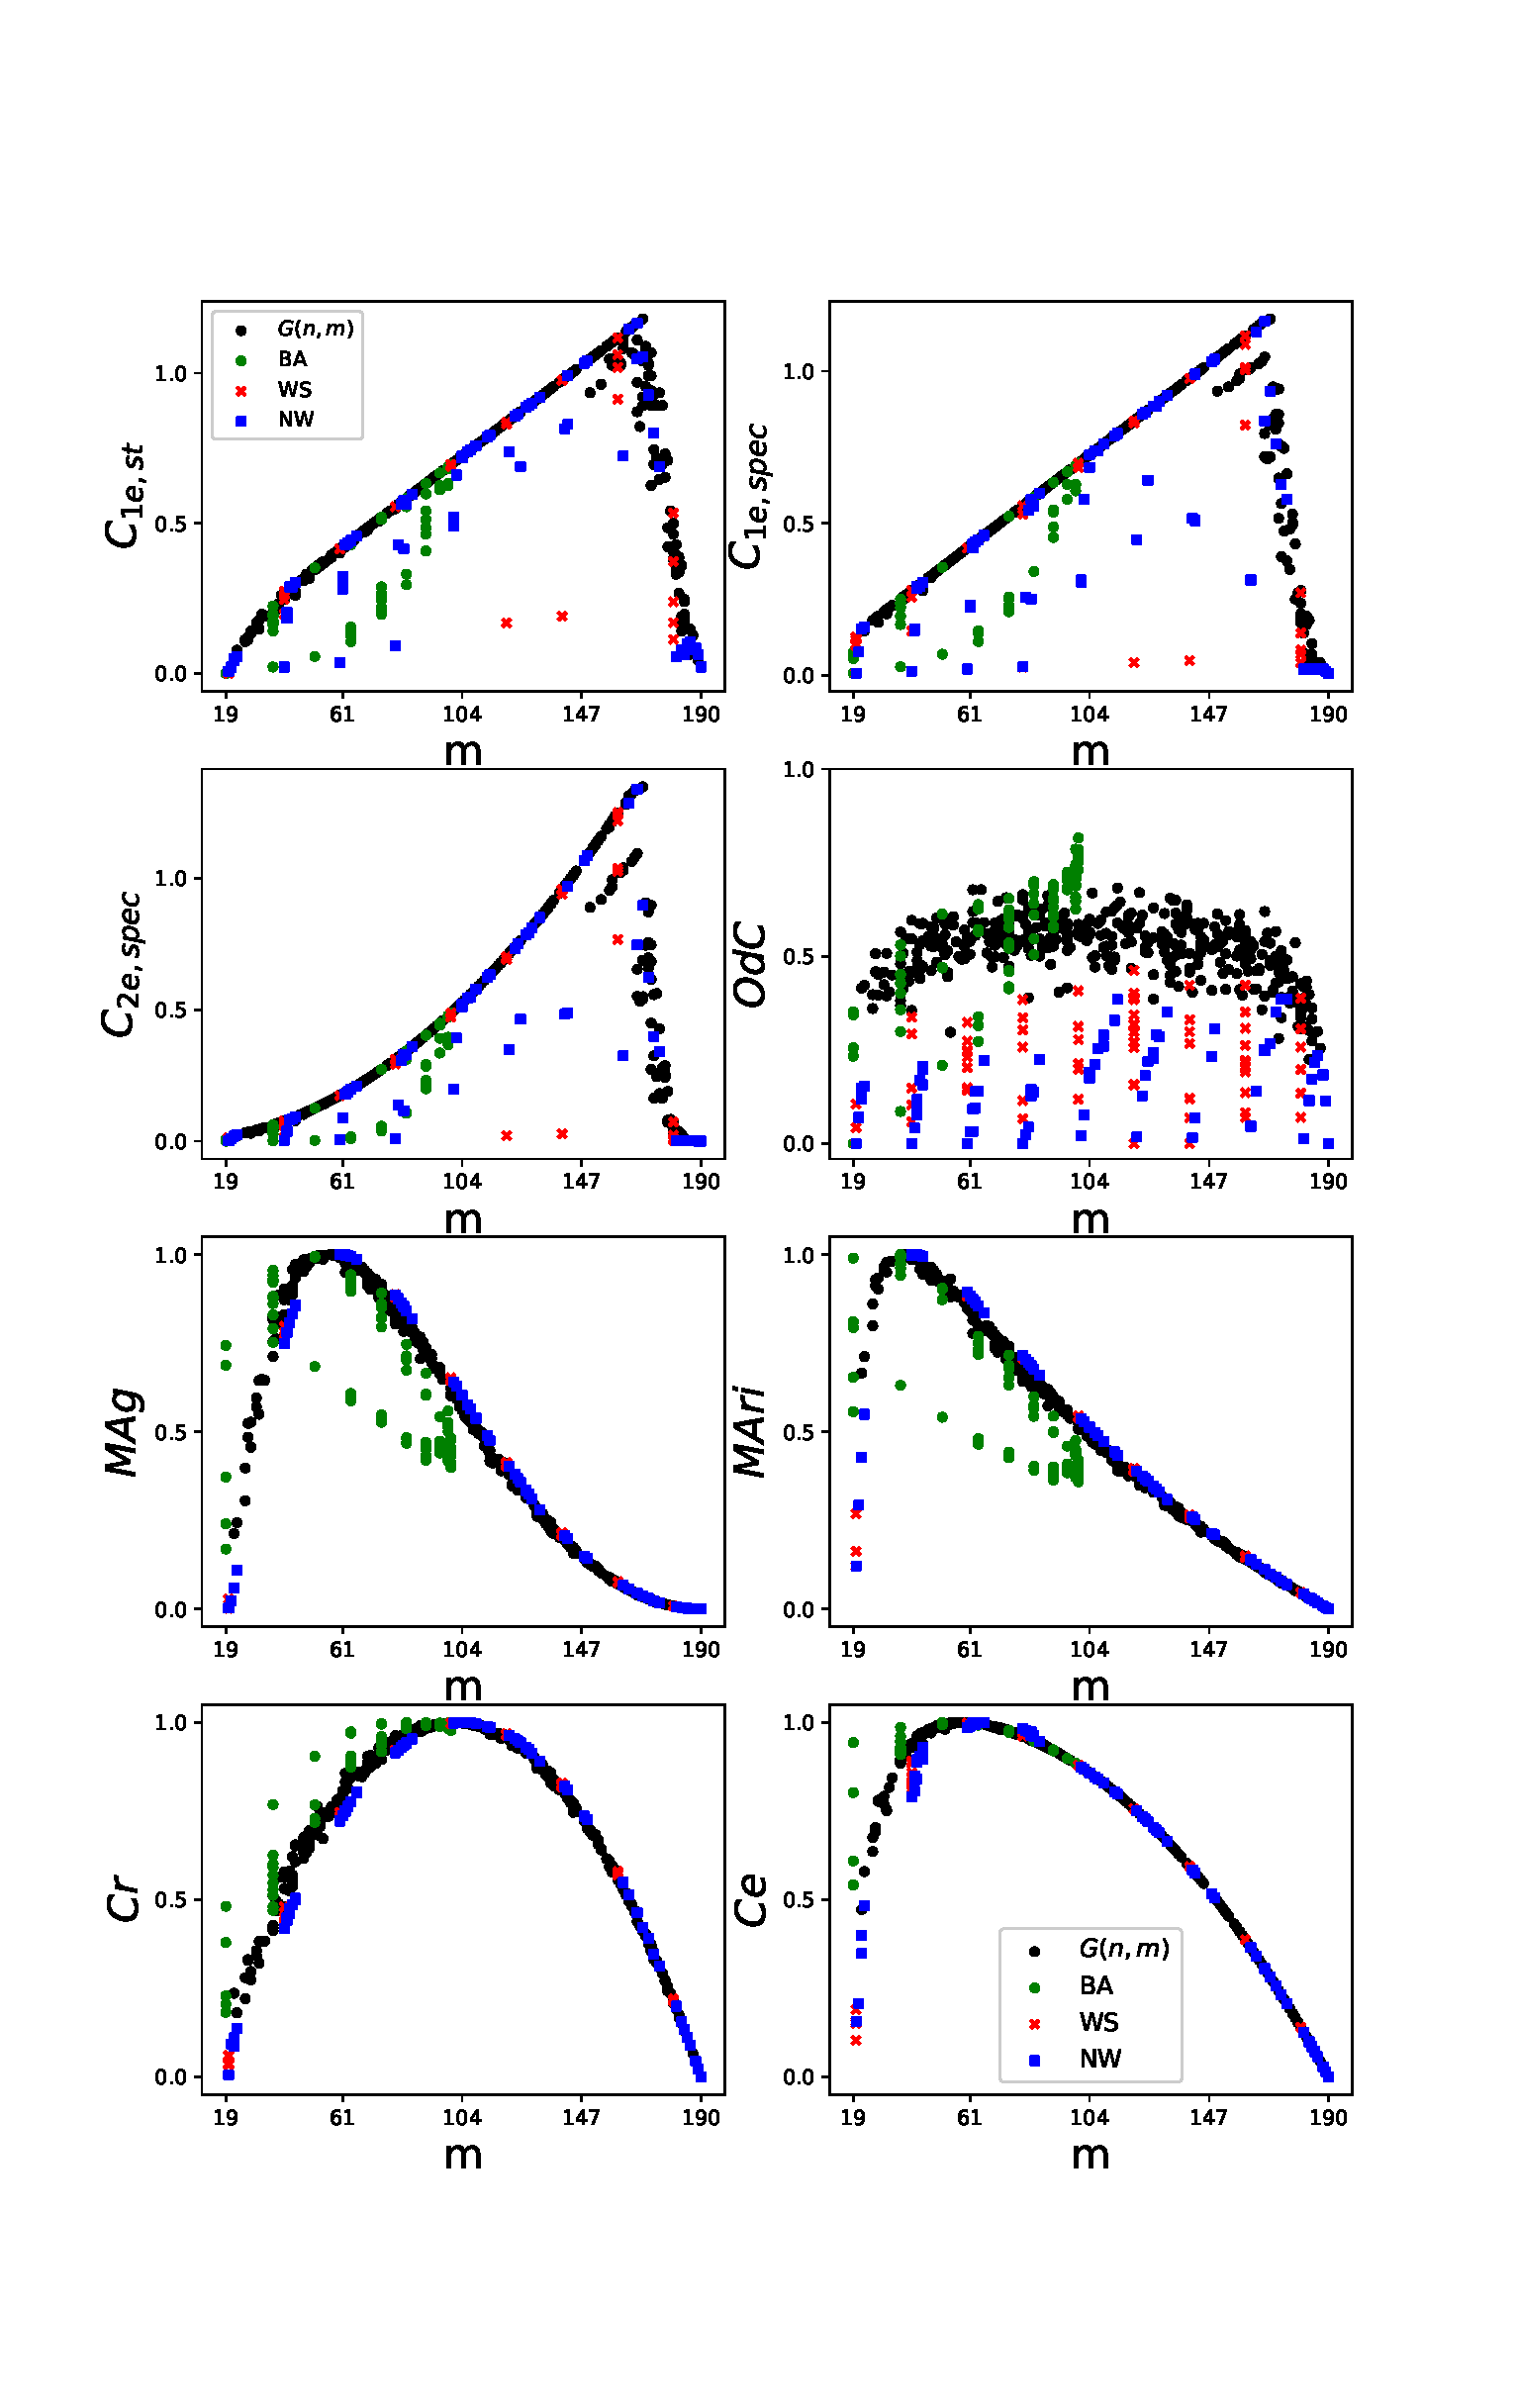
\includegraphics[width = 0.6\textwidth]{complexities_sp.eps}
    \label{fig:graph_models}
    \caption{Complexity of 500 $G(n,m)$ graphs, 100 BA graphs, 100 WS graphs and 100 NW graphs, all graphs have 20 nodes. Graphs are generated according to section \ref{generate_graphs}.}
\end{figure}
As informed in section \ref{problem}, different subgraph measures have normalisation problem and the complextity would exceed 1.\\
Surprisingling, diffrent subgraph measures and product measures are struggling to seperate random graphs, WS graphs and NW graphs. Only $OdC$ seperates random graphs and WS,NW model by giving random graphs higher complexity than WS and MW model with fixed $m$. This is because $OdC$ awards graphs with complicated degree correlation. On the other hand, WS and NW model generate graphs that have small degree difference between each node.\\
BA graphs give more intrersting results. Different subgraph measures assign lower complexity to BA graphs compare to random graphs. This can be caused by the preferential attachment. Preferential attachment ensures most nodes have low degree and builds hubs(nodes with high degree) in the graph. After cutting an edge/two edges between hubs and nodes with small degree, there is a high chance an isomorphic subgraph can be found, thus lower the complexity of the graph. In another word, subgraphs resulted by cutting the edge between hubs and node with small degree are very similar and occassionally isormophic.\\
$MA_g$ and $MA_{RI}$ perform similarly by assigning BA graphs lower value towards medium number of links. Both measures are depening on the variable $\sum_{i,j>i}d_id_j$. BA graphs ususally have less $\sum_{i,j>i}d_id_j$ because they are highly structure, causing less sum than a random graph. Contrarily, $Ce$ and $Cr$ cannot distinguish BA graphs and random graphs. $Ce$ is based on the efficiency of a graph, a highly complex graph should have small average distance with not too much links simultaneously. BA graph does not perform different than random graphs in $Ce$ measure.\\

\subsection{Complexity correlation}
Different type of measures focus on different properties/parameters of a network, monitor the correlation between measures will help us to further understand the behaviour on each measure. For this reason, we choosed three measures($C_{1e,st}$,$OdC$ and $MA_{RI}$) and monitored their behaviours on random and BA graphs.\\
\begin{figure}[ht]
    \label{fig:correlation}
    \centering
    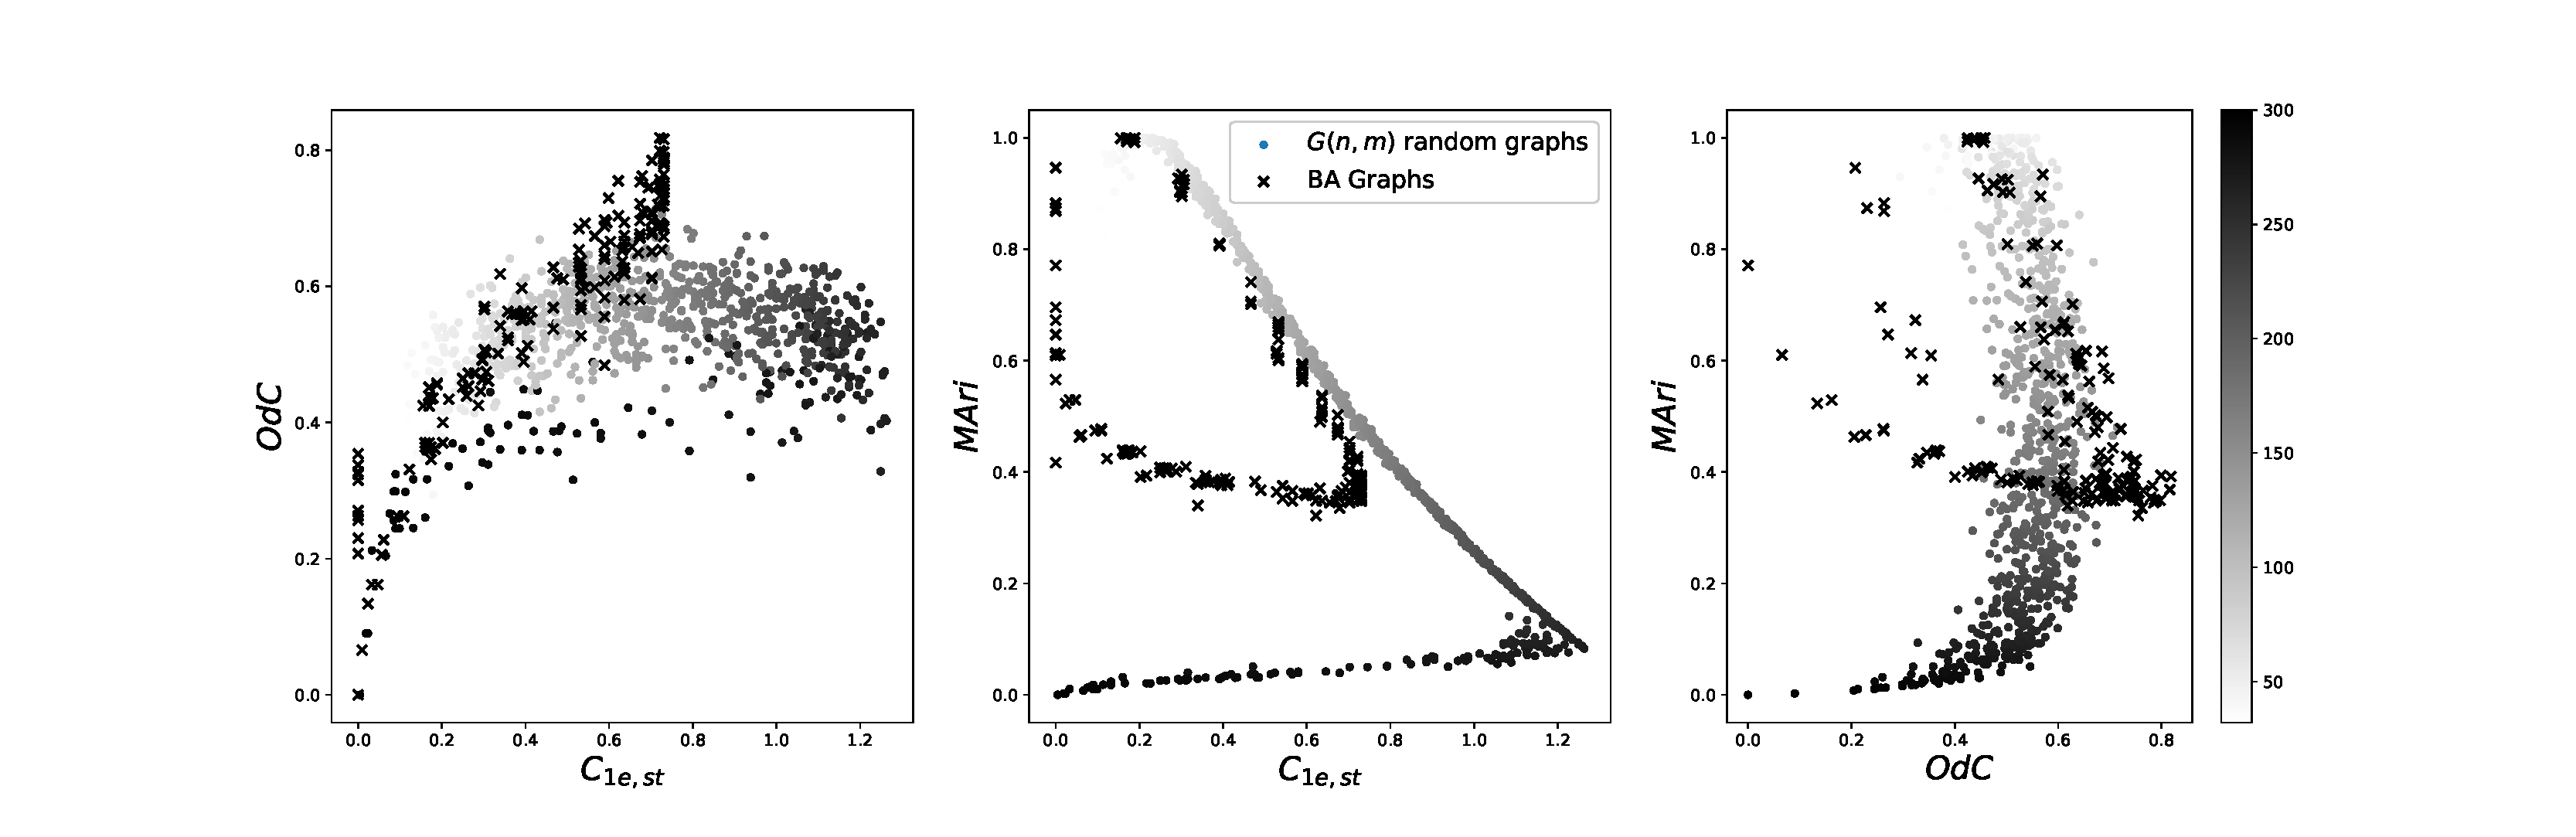
\includegraphics[width = 1.2\textwidth]{complexity_correlation.eps}
    \caption{Correation of complexity measures on random graphs and BA graphs with $n=25$. Generated according to the rules stated in section \ref{generate_graphs}. Colorbar represents change of $m$: higher the $m$, darker the datapoints.}
\end{figure}

\noindent
On random graphs, change of $OdC$ is not obvious, in figure \ref{fig:correlation}, $OdC$ values are spreaded whereas $C_{1e,st}$ increses as $m$ increses. In contrast, $OdC$ value of BA graphs increase as $C_{1e,st}$ value increases. 


\subsection{Complement graphs}
Definition of a complement graph is fairly simple: an edge list is created using a set contains all possible edges subtract the edges in the original graph. Analysing the complexity correlation between the original graph and the complement graph give us more inspirations of the measure. We have choose three different measures with different types: $OdC$, $MA_{RI}$ and $C_{1e,spec}$.
\begin{figure}[ht]
    \centering
    \label{fig:complement}
    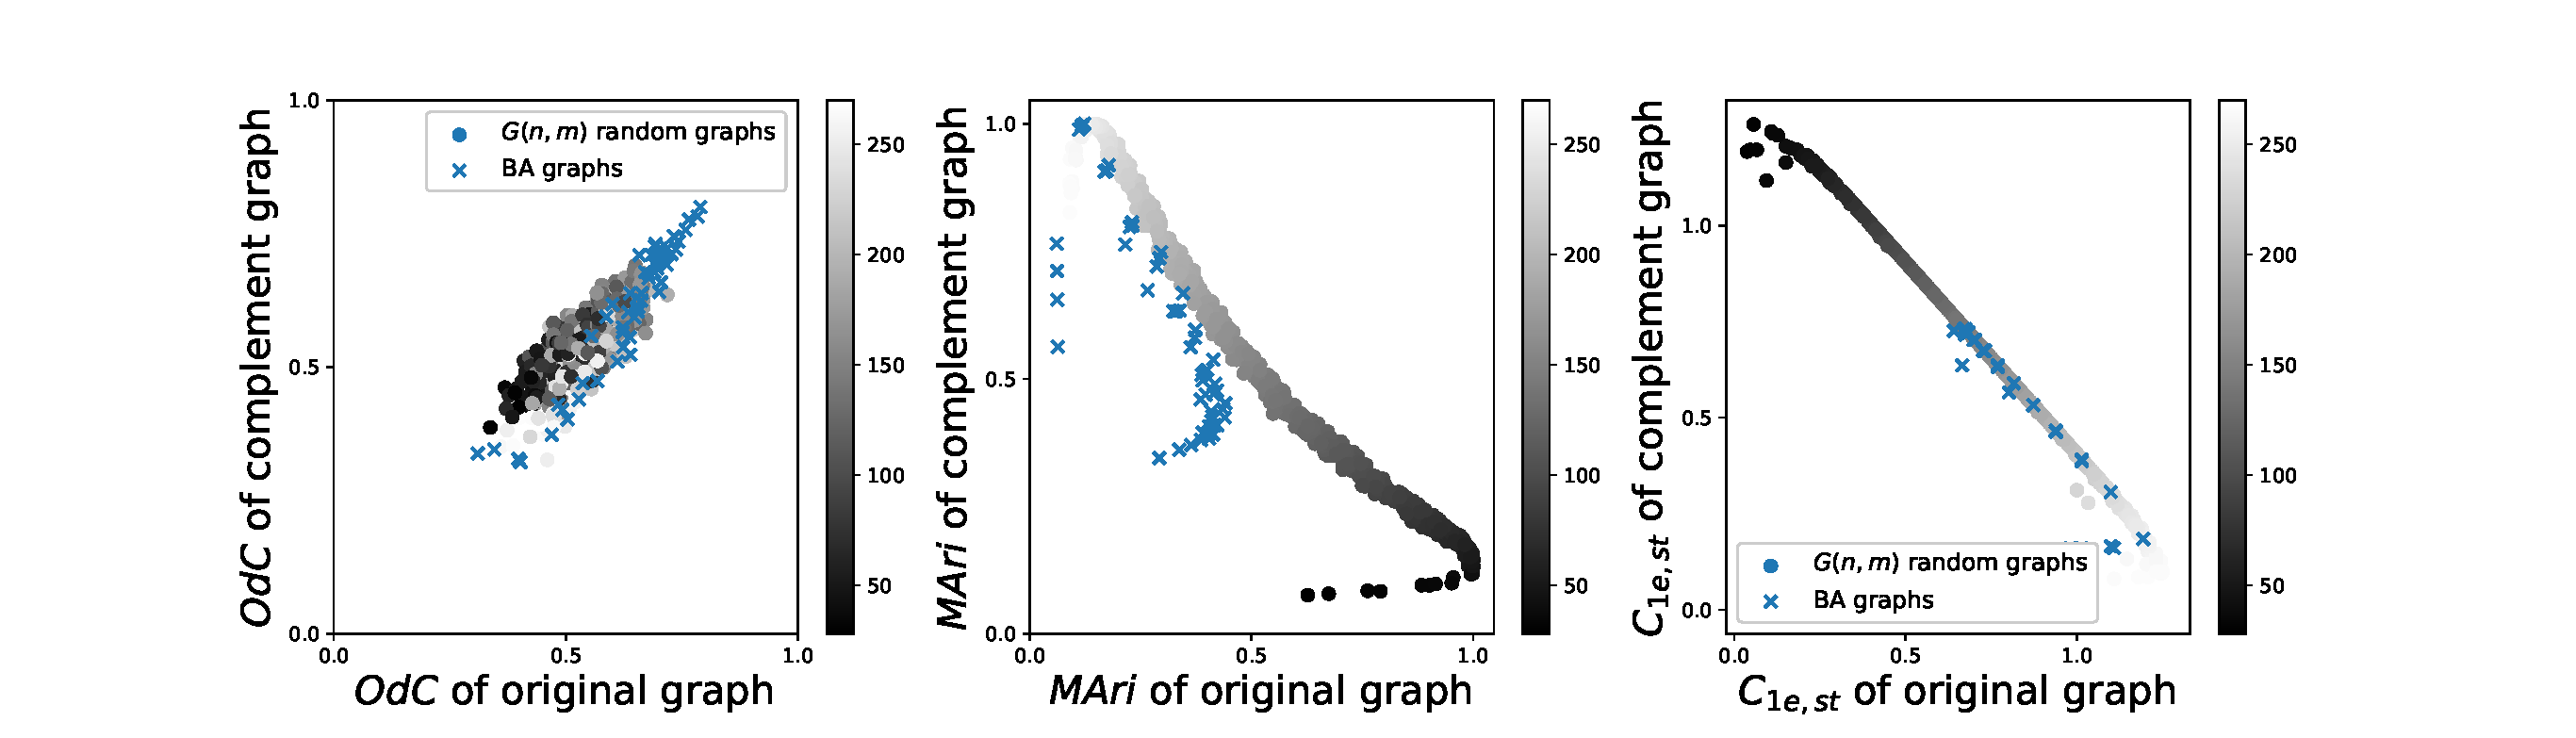
\includegraphics[width = \textwidth]{complement.eps}
    \caption{Complexities of the original graphs and complement graphs with $n=20$. There are two types of graphs are generated: 500 $G(n,m)$ random graphs and 100 BA graphs.}
\end{figure}

\subsection{$MA_{RI}$ on real networks}
To test our new measure $MA_{RI}$, 12 real networks are collected. To ensure comprehensive evaluation, various types of networks are used. To be applicable, we collected and processed bus networks in 6 cities. Bus networks are very different to other real networks. Bus networks contain extraordinary amount of nodes with degree 2. For simplification and general interest, we also inroduced modified bus networks. In modified bus networks, all nodes with $k=2$ are removed, whereas the edges are preserved. For instance, node $b$ is only conneted to $a$ and $c$. Node $b$ will be removed and a new edge $(a,c)$ will be added to the network. This will significantly decrease the distance of bus networks. Moreover, generated graphs are also added to be evaluated and compared.\\


\begin{table}[ht]
    \noindent\makebox[\textwidth]{
        \begin{tabular}{|c|c|c|c|c|c|c|c|}
            \hline
            Label & Name & Type & n & m& L & $L_r$ &$MA_{RI}$\\
            \hline
            \multicolumn{8}{|c|}{Real networks}\\
            \hline
            1 &  Dolphins\cite{dolphins} & Animal interaction & 62 & 159 & 3.357 & 2.524 & 0.999\\
            \hline
            2 &  PDZBase \cite{pdzbase}& protein interaction & 161 &209 & 5.326 & 5.326 & 0.824\\
            \hline
            3&  Hamsterster\cite{hamster} & Online social network & 874 & 4003 & 3.217 & 3.058 & 0.963\\
            \hline
            4& Roget's Thesaurus \cite{roget}& Thesaurus network &994 & 3640 & 4.075 & 3.466 & 0.960\\
            \hline
            5 & Flight\cite{flight} & Public transport & 3397 & 19230 & 4.103 & 3.350& 0.948\\
            \hline
            6 & UK train \cite{GBPT}& UK train network & 2490 & 4377 & 10.384&6.220 & 0.664\\
            \hline
            \multicolumn{8}{|c|}{Bus networks}\\
            \hline
            7&\multicolumn{2}{c|}{London}&8653&12285&32.338&8.687&0.38\\ 
            \hline
            8&\multicolumn{2}{c|}{Paris}&10644&12309&47.631&11.059&0.173\\ 
            \hline
            9&\multicolumn{2}{c|}{Berlin}&4316&5869&33.284&8.366&0.358\\ 
            \hline
            10&\multicolumn{2}{c|}{Sydney}&22659&26720&36.131&11.688&0.173\\ 
            \hline
            11&\multicolumn{2}{c|}{Detroit}&5683&5946&70.513&11.708&0.062\\ 
            \hline
            12&\multicolumn{2}{c|}{Beijing}&9249&14058&27.891&8.214&0.441\\ 
            \hline
            \multicolumn{8}{|c|}{Modified Bus}\\
            \hline
            13&\multicolumn{2}{c|}{London}&3417&6018&18.308&6.462&0.553\\ 
            \hline
            14&\multicolumn{2}{c|}{Paris}&2762&4301&15.386&6.975&0.468\\ 
            \hline
            15&\multicolumn{2}{c|}{Berlin}&1662&2941&18.36&5.867&0.586\\ 
            \hline
            16&\multicolumn{2}{c|}{Sydney}&4834&8358&17.665&6.838&0.49\\ 
            \hline
            17&\multicolumn{2}{c|}{Detroit}&295&483&6.341&4.794&0.643\\ 
            \hline
            18&\multicolumn{2}{c|}{Beijing}&4072&8325&14.864&5.902&0.64\\ 
            \hline
        \end{tabular}
    }
    \caption{Label and description of used networks} 
    \label{tb:descriptions}
\end{table}


\begin{figure}[ht]
    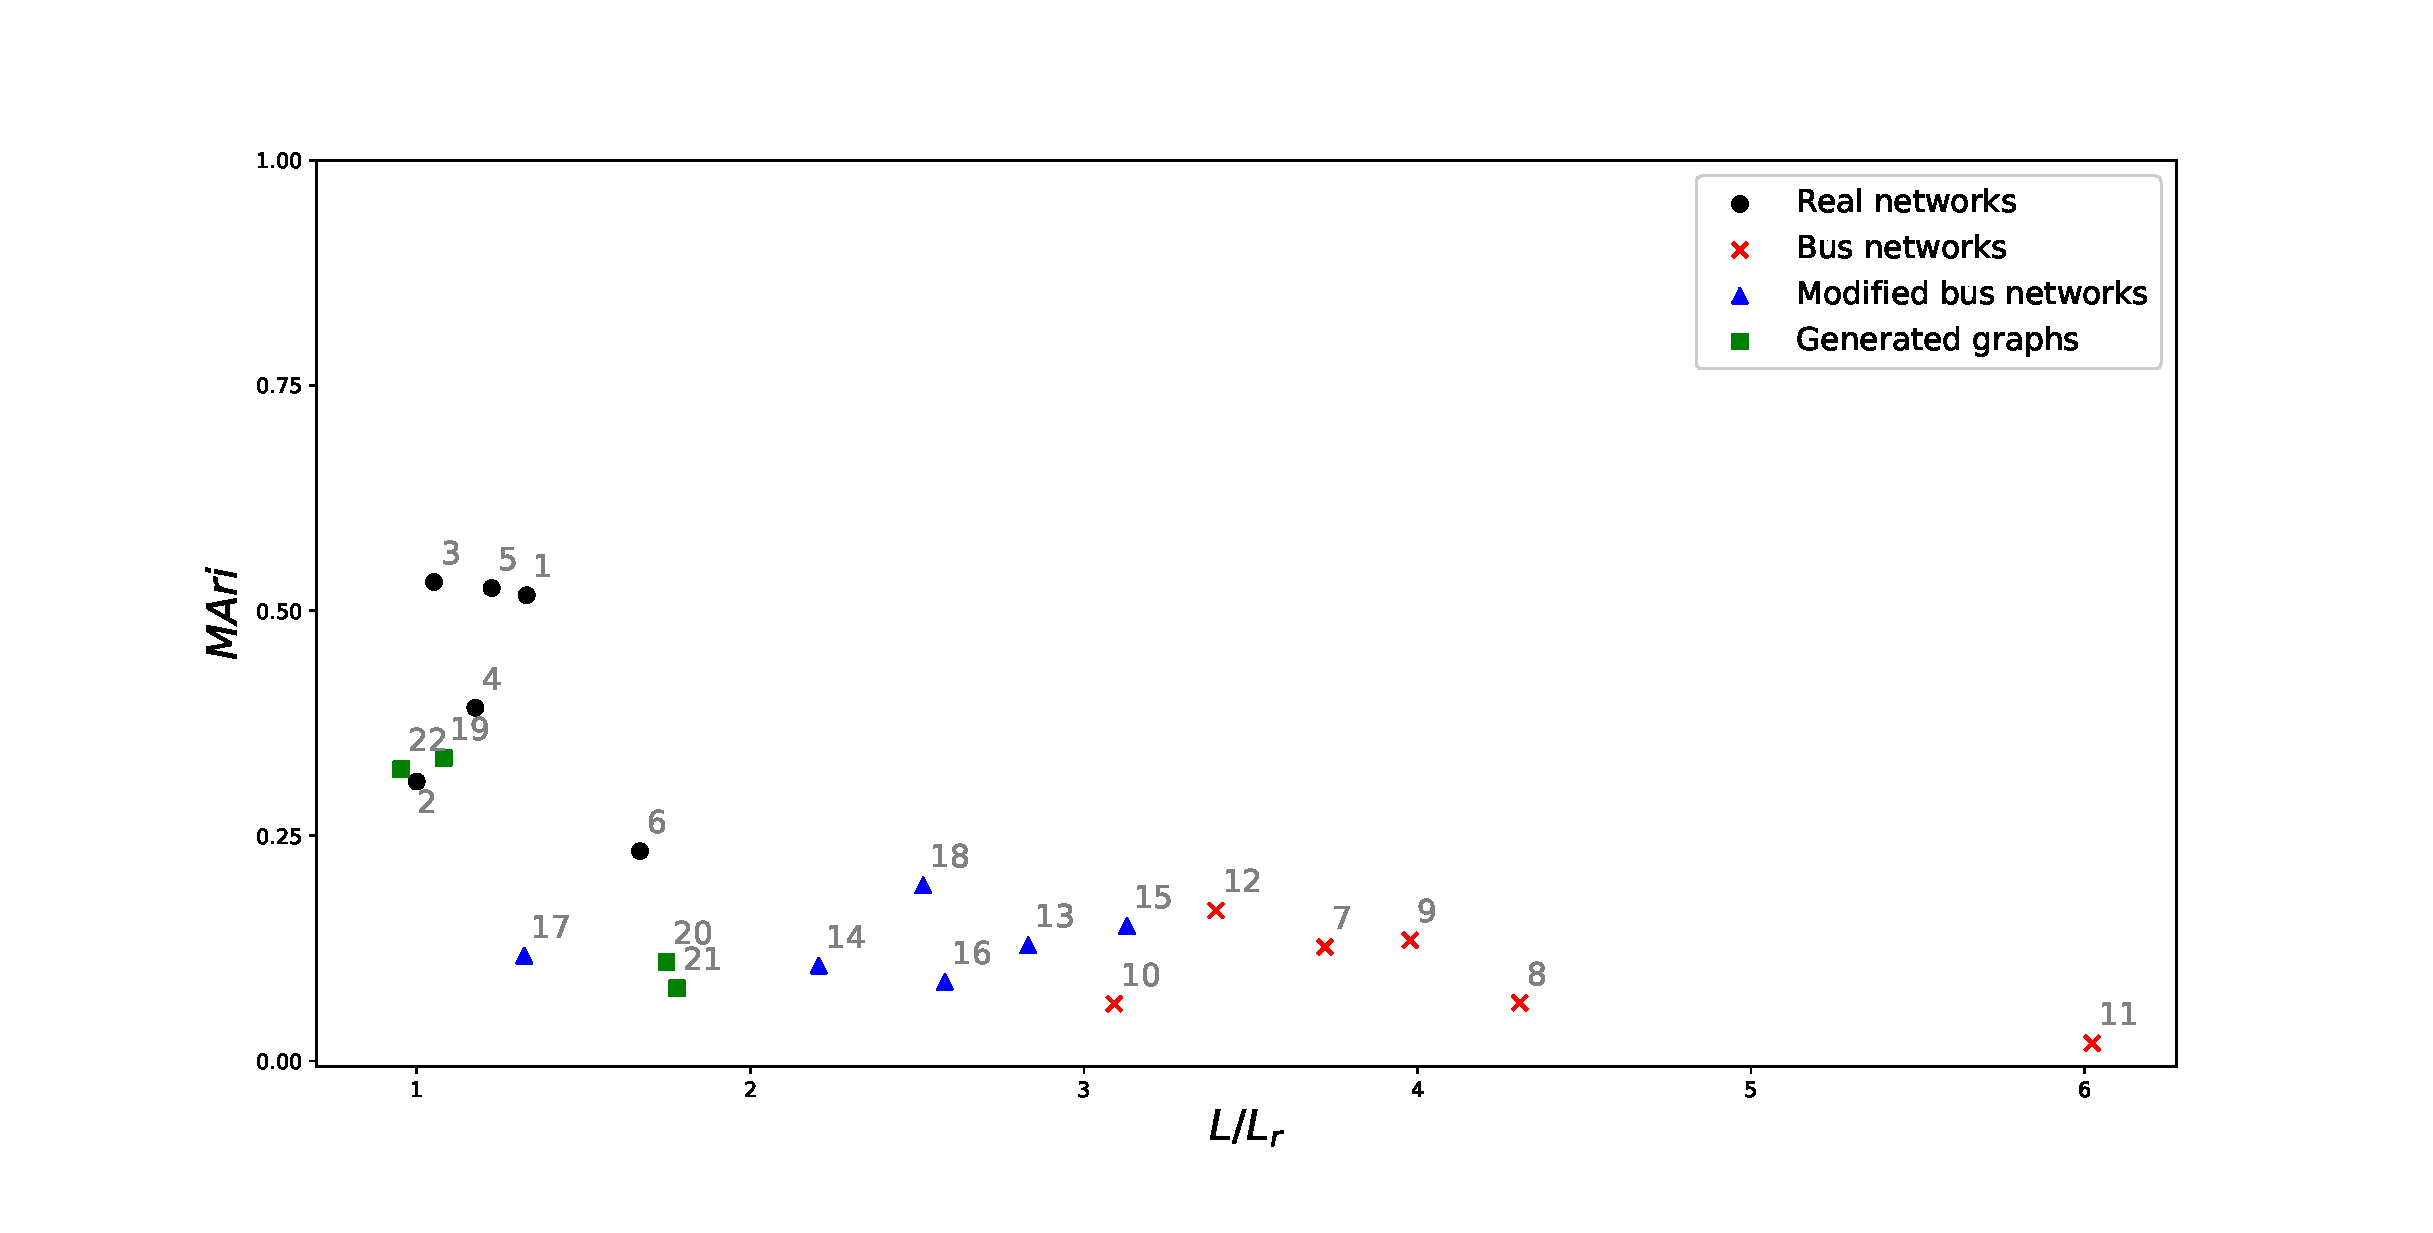
\includegraphics[width = \textwidth]{real_networks.eps}
    \caption{$MA_{RI}$ complexity of real networks, bus networks, modified bus networks and graphs generated by graph models, labelling and description can be found in table \ref{tb:descriptions}.}
    \label{fig:real_networks}
\end{figure}
After careful consideration, we choosed average distance ratio $L/L_r$ to be the variable showin on x-axis in figure \ref{fig:real_networks}. We decided that the average distance is a more important parameter to consider about. As suggested, all the bus networks have significantly higher average distance ratio. Even after modified, the average distance ratios are still relatively high. But higher average distance ratio brings less $MA_{RI}$ complexity. We can suggest a negative correlation between the average distance ratio and the $MA_{RI}$ complexity. There is an exception of real networks, which is the UK train network. Cosidering the similarity between bus networks and train networks, it should not be a big surprise. Generated graphs also behaves similar to standard real networks; low average distance ratio with high complexity, as they are intended to simulate the behaviour of standard real networks.\\
To discuss the cause of increase of $MA_{RI}$ complexity after modified, we need to consider about the parameter $MA_{RI}$ focusing on. $\sum_{i,j>i}d_id_j$ is the only variable that affects the complexity of a graph. The essence of the measure is calculating the average $d_id_j$. By removing nodes with degree 2, average $d_id_j$ will be increased, and leads to an increase of the $MA_{RI}$ complexity.

\subsection{Rewiring on real networks}
As recommened in section \ref{rewiring}, rewiring is an important technique to monitor the behaviour of a network. Hence, we rewired real networks and modified bus networks to record their behaviour. Both single link rewiring and pairwise rewiring will be used. The reason we are going to use $OdC$ instead of $MA_{RI}$ is that pairwise rewiring will keep the degree distribution, and $MA_{RI}$ cannot detect unchanged degree.
\begin{figure}[ht]
    \centering
    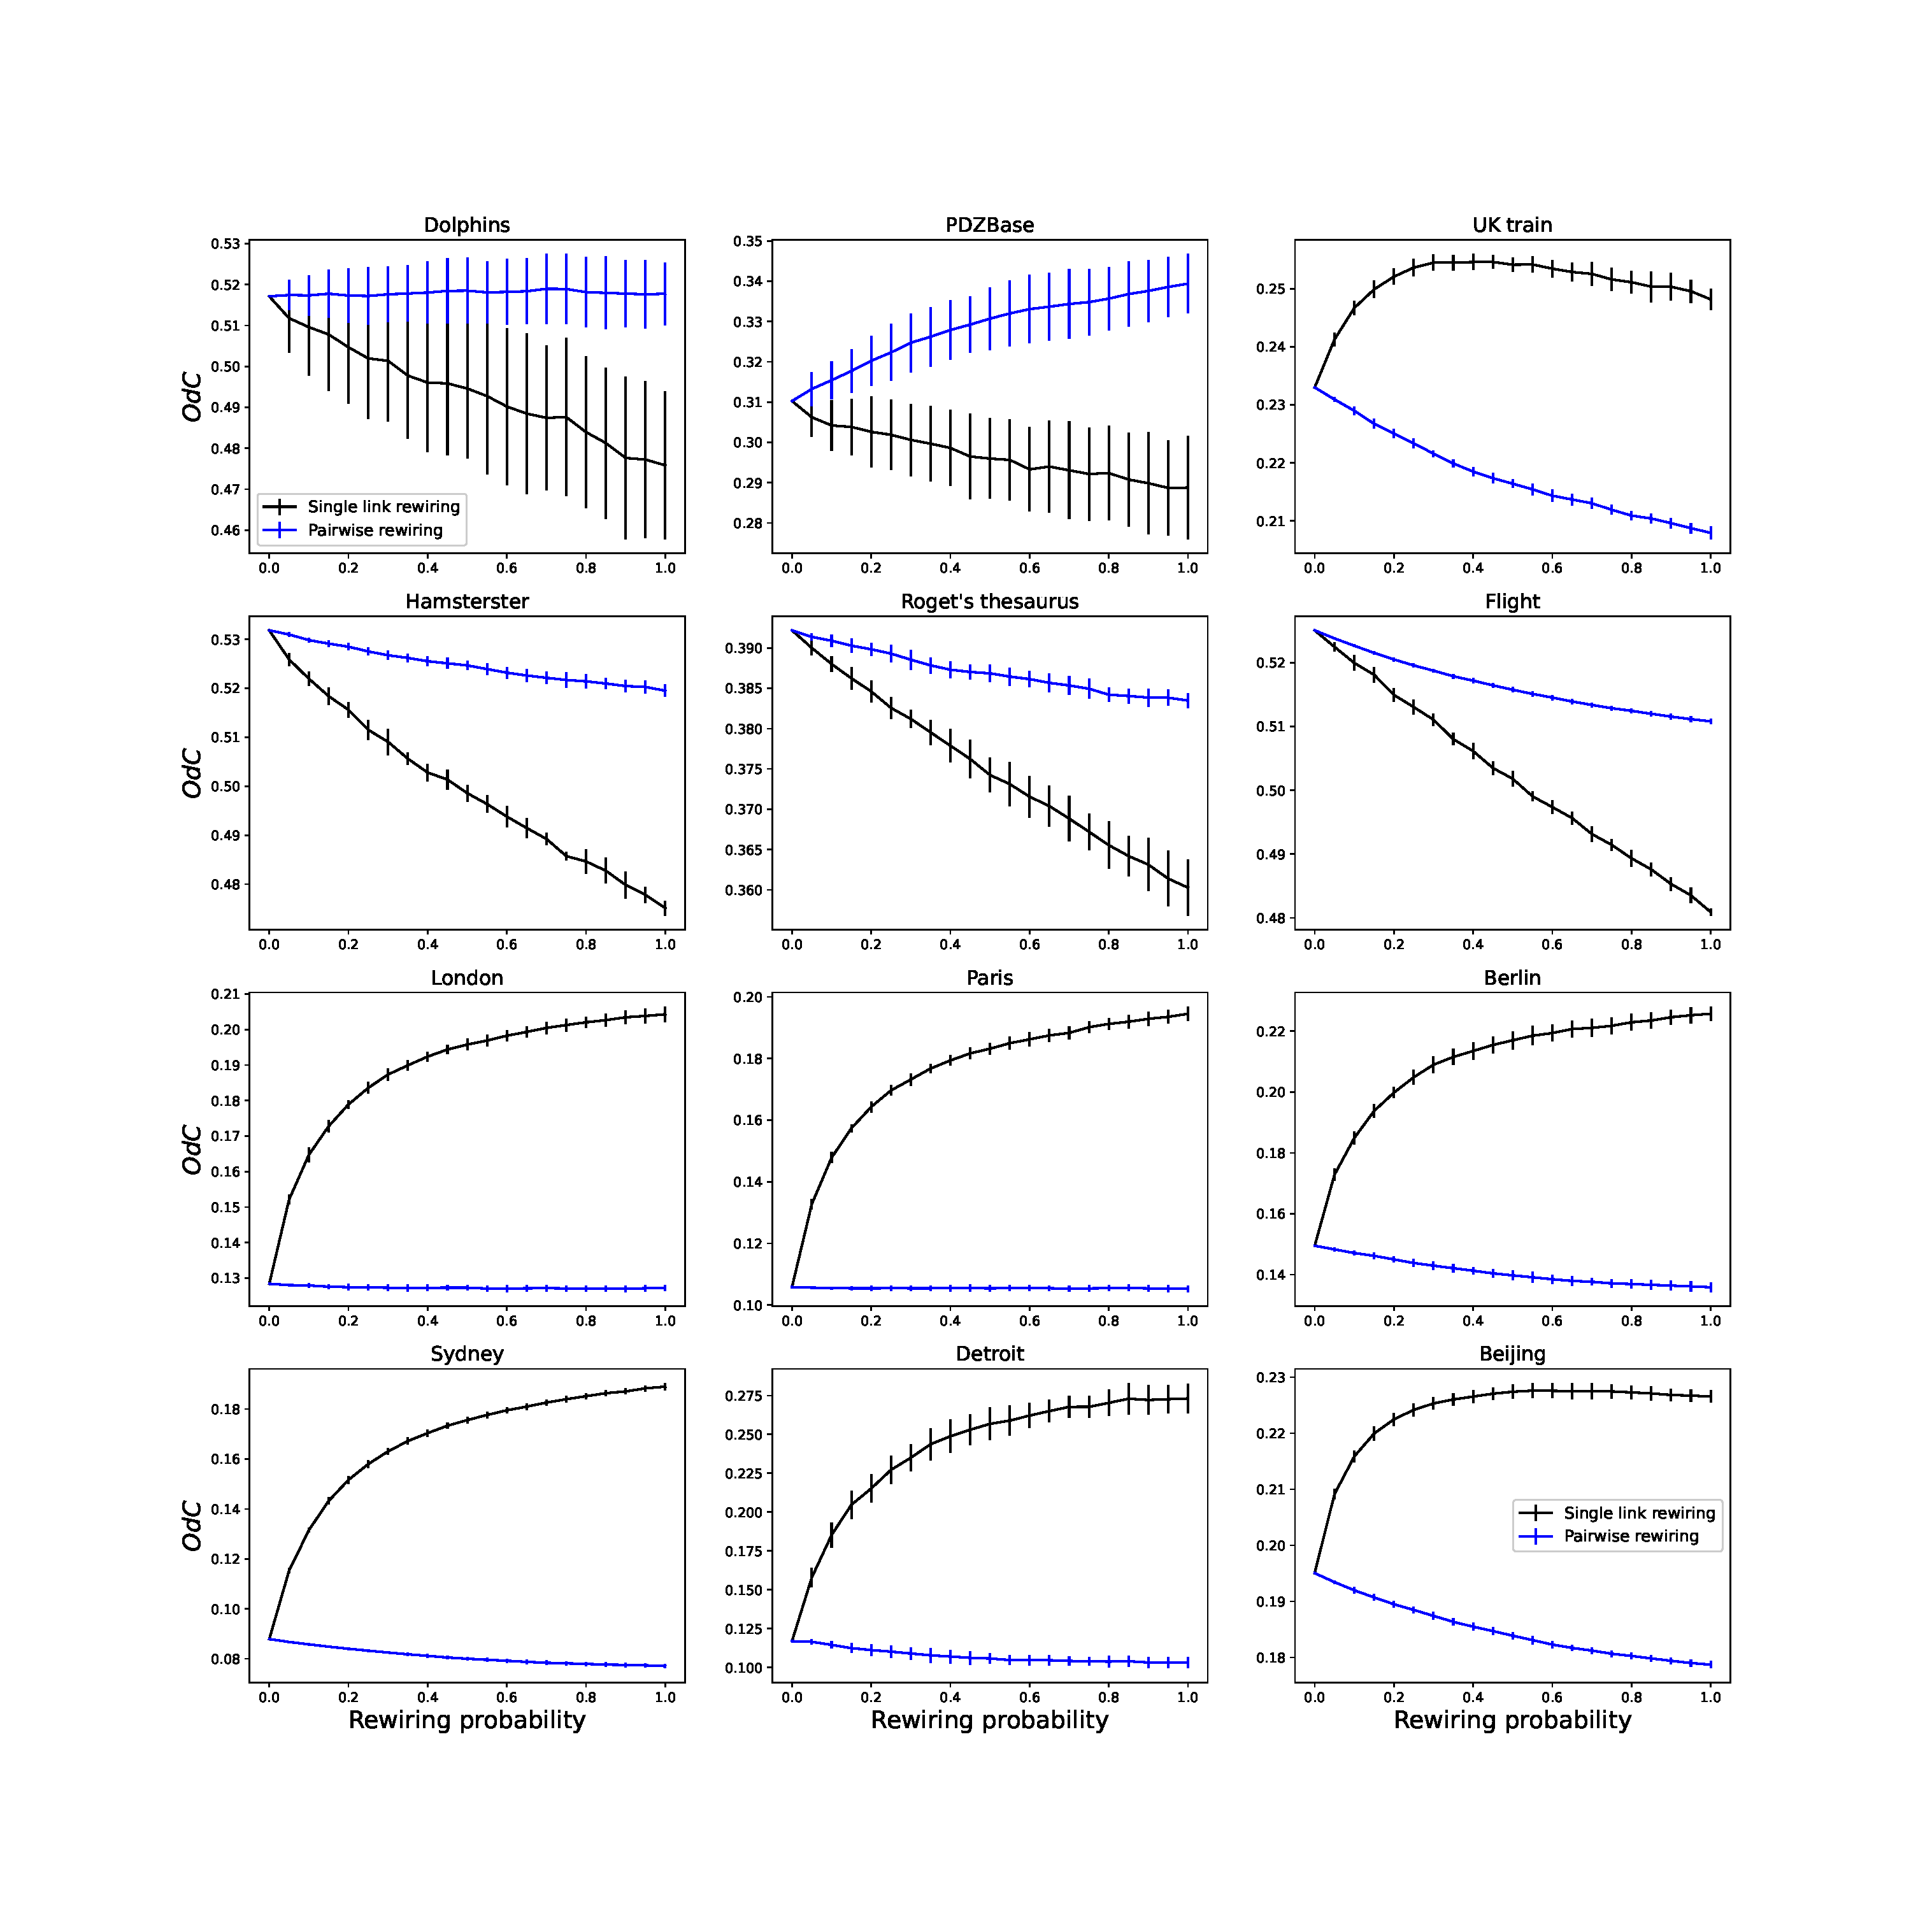
\includegraphics[width=\textwidth]{rewiring.eps}
    \caption{Change of complexity respect to rewiring porobability.}
\end{figure}


\clearpage
\section{Conclusion}

\printbibliography

\end{document}
